\documentclass[preprint, authoryear, 12pt]{elsarticle}
\usepackage{amsmath}
\usepackage{amssymb,amsfonts, amsthm}
\pdfoutput=1 %for arXiv
\pdfminorversion=4
% uncomment the line below if you want 2 cm margins instead of wide margins - wide margins are 1in
%2 cm are smaller than 1in, so see what works after final version ready
\usepackage[margin=2cm,heightrounded=true,centering]{geometry}

\tolerance=2000 
\emergencystretch=20pt 

\usepackage{float}
\usepackage{listings}
\usepackage{mathrsfs}
\usepackage{amscd}
\usepackage{verbatim}
\usepackage{euscript}


\usepackage{comment}

%\usepackage{appendix}
\usepackage{etoolbox}

% Inserts \clearpage before \begin{appendices}
\BeforeBeginEnvironment{appendices}{\clearpage}


\usepackage{setspace}
%\doublespacing


\usepackage{soul}
\usepackage{lineno}
\usepackage{graphicx}
\usepackage{caption}
\usepackage{subcaption}
\usepackage{float}
\usepackage[shortlabels]{enumitem}
% dont use \usepackage{tilting} with elsevier
\usepackage{blindtext}
% \usepackage{mymacros}
\usepackage{comment}
\usepackage{natbib}
\usepackage{mathtools}
\usepackage{multirow}
\usepackage{bbm}
\mathtoolsset{showonlyrefs=true}
\usepackage{bm}
\usepackage[usenames, dvipsnames]{color}
\definecolor{cre}{rgb}{0.39, 0.05, 0.05}
\usepackage{wrapfig}

\usepackage{booktabs}
\newcommand{\bftab}{\fontseries{b}\selectfont}
%\usepackage{bold-extra}
% \usepackage{fixltx2e} for text subsetting: \textsubscript{}


\usepackage{caption}

%\DeclareCaptionFont{mysize}{\fontsize{8}{9.6}\selectfont}
%\captionsetup{font=mysize}



\usepackage{indentfirst}
\usepackage{longtable}

\usepackage{xpatch} \makeatletter \xpretocmd \start@align{\linenomathWithnumbers}{}{\fail}

\makeatletter
\def\thanks#1{\protected@xdef\@thanks{\@thanks
        \protect\footnotetext{#1}}}
\makeatother

\renewcommand{\thesubfigure}{\Alph{subfigure}}


%\usepackage{titlesec}
%\renewcommand\thesection{\arabic{section}.} \renewcommand\thesubsection{\thesection\arabic{subsection}}

\usepackage[colorlinks = true,
            linkcolor = blue,
            urlcolor  = blue,
            citecolor = blue,
            anchorcolor = blue]{hyperref}


%\renewcommand\maketitlehooka{\null\mbox{}\vfill}
%\renewcommand\maketitlehookd{\vfill\null}
\newsavebox\CBox
\def\textBF#1{\sbox\CBox{#1}\resizebox{\wd\CBox}{\ht\CBox}{\textbf{#1}}}
%%%%%%%%%%%%%%%%%%%%%%%%%%%%%%%%%%%%%%%%%%%%%%%%%%%%%%
%%%%%%%%%%%%%%%%%%%%%%%%%%%%%%%%%%%%%%%%%%%%%%%%%%%%%%
%%%%%%%%%%%%%%%%%%%%%%%%%%%%%%%%%%%%%%%%%%%%%%%%%%%%%%
%%%%%%%%%%%%%%%%%%%%%%%%%%%%%%%%%%%%%%%%%%%%%%%%%%%%%%
% 				BEGIN DOCUMENT
%%%%%%%%%%%%%%%%%%%%%%%%%%%%%%%%%%%%%%%%%%%%%%%%%%%%%%
%%%%%%%%%%%%%%%%%%%%%%%%%%%%%%%%%%%%%%%%%%%%%%%%%%%%%%
%%%%%%%%%%%%%%%%%%%%%%%%%%%%%%%%%%%%%%%%%%%%%%%%%%%%%%
%%%%%%%%%%%%%%%%%%%%%%%%%%%%%%%%%%%%%%%%%%%%%%%%%%%%%%
\usepackage{epstopdf}
\epstopdfDeclareGraphicsRule{.tif}{jpg}{.jpg}{convert #1 \OutputFile}
\AppendGraphicsExtensions{.tif}
\epstopdfDeclareGraphicsRule{.TIF}{jpg}{.jpg}{convert #1 \OutputFile}
\AppendGraphicsExtensions{.TIF}
\journal{Progress in Oceanography (William T. Peterson Special Issue)}
%\renewcommand*{\today}{July 13, 2020}
\setlength{\bibsep}{0pt plus 0.3ex}
\begin{document}
%\linenumbers
%\maketitle
\begin{frontmatter}
\title{Capturing Copepod Dynamics in the Northern California Current Using Sentinel Stations}

\author[1]{Michael Dumelle\corref{cor1}}
\ead{dumellem@oregonstate.edu}
\author[2]{Jesse F. Lamb}
\author[3]{Kym C. Jacobson}
\author[3]{Mary Hunsicker}
\author[4]{Cheryl A. Morgan}
\author[5]{Brian J. Burke}
\author[3]{William T. Peterson}

\cortext[cor1]{Corresponding author}
\address[1]{Department of Statistics, Oregon State University, Corvallis, OR 97331}
\address[2]{Fisheries-Oceanography Coordinated Investigations, National Marine Fisheries Service, Alaska Fisheries Science Center, Seattle, WA 98115, USA}
\address[3]{Fish Ecology Division, National Marine Fisheries Service, Northwest Fisheries Science Center, Newport, OR 97365, USA}
\address[4]{Cooperative Institute for Marine Resources Studies, Hatfield Marine Science Center, Oregon State University, Newport, OR 97365, USA}
\address[5]{Fish Ecology Division, National Marine Fisheries Service, Northwest Fisheries Science Center, Seattle, WA 98112, USA}

\begin{abstract}
Ecosystem indicators track information about states and trends in ocean systems and are a valuable tool for ecosystem assessment and management.  To ensure that indicators are used appropriately in both science and management contexts, it is important to understand the extent to which they represent broader spatial patterns.  In the Northern California Current (NCC) off the Oregon and Washington state coasts in the USA, copepod metrics derived from data collected at a well-sampled station on the Newport Hydrographic (NH) Line (‘NH05’, five nmi offshore from Newport, OR, USA) are commonly used as indicators of the region’s general ocean conditions.  Using correlation analyses, we examined the utility of NH05 as a sentinel station (i.e. representative of a broader region) with respect to the abundance and biomass of warm-water and cold-water copepods in the NCC.  Copepod correlations between NH05 and other locations in the NCC were higher for the warm-water copepods than the cold-water group, with correlations being slightly higher for abundance than biomass. \textit{Paracalanus parvus} had the highest NH05 correlations among the warm-water copepod species, and \textit{Acartia longiremis} had the highest NH05 correlations among the cold-water copepod species. We also broadened our analysis to evaluate other sampling sites as sentinel stations and found that some sites were equally or more representative of copepod dynamics in the NCC than NH05, though none of these sites tend to be sampled as often as NH05.  This analysis emphasized that the warm-water copepods tend to be more similarly distributed in the NCC than the cold-water copepods, and thus their changes through time are better captured by most stations.  In contrast, correlations among the cold-water copepods in the NCC vary by location and appear to be strongly related to depth, with the highest correlations at mid-shelf stations.  
\end{abstract}

\begin{keyword}
Abundance \sep Biomass \sep Climate \sep Correlation \sep Newport Hydrographic Line  \sep Zooplankton
\end{keyword}
\end{frontmatter}
%%%%%%%%%%%%%%%%%%%%%%%%%%%%%%%%%%%%%%%%%%%%%%%%%%%%%%
%%%%%%%%%%%%%%%%%%%%%%%%%%%%%%%%%%%%%%%%%%%%%%%%%%%%%%
%        ABSTRACT
%%%%%%%%%%%%%%%%%%%%%%%%%%%%%%%%%%%%%%%%%%%%%%%%%%%%%%
%%%%%%%%%%%%%%%%%%%%%%%%%%%%%%%%%%%%%%%%%%%%%%%%%%%%%%



%%%%%%%%%%%%%%%%%%%%%%%%%%%%%%%%%%%%%%%%%%%%%%%%%%%%%%
%%%%%%%%%%%%%%%%%%%%%%%%%%%%%%%%%%%%%%%%%%%%%%%%%%%%%%
%        INTRODUCTION
%%%%%%%%%%%%%%%%%%%%%%%%%%%%%%%%%%%%%%%%%%%%%%%%%%%%%%
%%%%%%%%%%%%%%%%%%%%%%%%%%%%%%%%%%%%%%%%%%%%%%%%%%%%%%

\clearpage
\section{Introduction}

Ocean scientists rely on survey data to gather information about key environmental variables and ecosystem processes. But it is often unfeasible to consistently sample the entire temporal or spatial domain. Because of this challenge, it is common to use indicator metrics to capture behavior of a physical or biological system. It is important to understand how well indicator metrics represent broad temporal and spatial patterns in a region so that scientists and stakeholders can be adequately informed. Copepods are a commonly used indicator species of ocean conditions in the northern region of the California Current (NCC) because copepod bioenergetics can inform the bioenergetics for higher trophic levels \citep{peterson2014applied, tucker2015coastal, harvey2020importance}. In this paper, we use correlation analyses to inform copepod dynamics in the NCC. We focus on the representativeness of NH05, a historically well sampled station on the Newport Hydrographic (NH) Line five nautical miles (nmi) (5nmi = 9.3km) off the central Oregon Coast, USA.

The copepod community structure in the NCC fluctuates seasonally in response to local wind forcing and inter-annually in response to basin scale forcing. In shelf waters off central Oregon, copepod presence depends on advective transport: the presence of cold-water species indicates southward transport of subarctic waters, and the presence of warm-water species indicates northward or onshore transport of subtropical waters \citep{keister2011zooplankton}.   These different copepod communities provide distinct lipid classes and fatty acids to upper trophic levels \citep{miller2017temporal}. Lipid-rich neritic and subarctic copepods (cold-water copepods) are the dominant copepod taxa in the NCC during the summer upwelling season \citep{peterson2003interannual, hooff2006copepod, mackas2006zooplankton}. These cold-water copepods are typically from the Bering Sea and coastal Gulf of Alaska  \citep{cooney2001seasonality, mackas2001changes}. Lipid poor neritic and oceanic copepods (warm-water copepods) are common in the NCC when northerly upwelling winds subside and give rise to storm driven, southwesterly winds in fall and winter \citep{peterson1977seasonal}. These warm-water copepods are typically from the offshore Transition Zone and North Pacific Gyre or in the coastal waters of the Central California Current \citep{peterson1977seasonal}.  Basin-scale processes can also alter the copepod community structure in the NCC via the positive (warm) and negative (cold) phases of the Pacific Decadal Oscillation (PDO) along with El Niño and La Niña conditions \citep{peterson2003interannual, hooff2006copepod, mackas2006zooplankton, peterson2014applied, fisher2015impact, peterson2017pelagic}. During a negative phase PDO, there is increased equatorward transport of cold-water copepod species from the Gulf of Alaska to the coastal NCC. During a positive phase PDO, warm-water copepod species from oceanic and southern subtropical waters contribute an anomalously larger fraction of the copepod biomass in the NCC \citep{bi2011transport, keister2011zooplankton}. La Niña and El Niño conditions can also modify local winds and alongshore transport that results in higher abundances of cold-water and warm-water copepods, respectively, to the region \citep{fisher2015impact}.

Our understanding of coastal physical and biological oceanography in the NCC is heavily influenced by studies conducted on the NH Line.  Physical oceanography studies along the NH Line began in 1961 and continue today (\href{http://terra.oregonstate.edu/2018/02/towing-the-line/}{http://terra.oregonstate.edu/2018/02/towing-the-line/}).  Since 1996, zooplankton and hydrographic sampling have been conducted biweekly to monthly at seven stations along the NH Line (from 1 to 25 nmi, approximately 1.8 to 46 km, from shore). The most frequently sampled station along the NH Line is five nmi offshore and referred to as NH05 (44.67$^\circ$N, 124.17$^\circ$W). The depth at NH05 is around 60 m, so it is commonly referred to as a midshelf station. The high frequency sampling at NH05 yields several useful time series of oceanographic observations for many species including copepods.  Because of this, NH05 is often referred to as a “sentinel station” for the NCC, being informative of broad trends in the region. Several copepod community metrics at NH05  have successfully recorded seasonal, decadal, and extreme oceanographic events at both regional and basin scales \citep{mackas2006zooplankton, keister2011zooplankton, fisher2015impact, peterson2017pelagic, harvey2020importance}. Because copepods capture the bioenergetics of the lower food web, they can be used to develop indicators of nearshore marine conditions that are informative for marine fishes and other species \citep{peterson2014applied}. Indices gathered from NH05 are critical components in ecosystem status reports, such as the Annual State of the California Current \citep{wells2017state, thompson2018state, thompson2019state} and the California Current Integrated Ecosystem Assessment \citep{harvey2018ecosystem, harvey2019ecosystem}. These indices are used to inform William T. Peterson’s red-light, green-light ‘stop-light chart’, which provides stakeholders and managers an annual qualitative summary of “good” and “poor” ocean conditions encountered by juvenile Pacific salmon entering the nearshore Pacific Ocean \citep[][\href{https://www.nwfsc.noaa.gov/oceanconditions}{https://www.nwfsc.noaa.gov/oceanconditions}]{peterson2014applied}.

Comparisons of interannual biomass anomalies of warm-water copepods, cold-water copepods, and species richness have demonstrated that NH05 is representative of broader ocean conditions off the Pacific Northwest coast \citep{mackas2004comparisons, mackas2006zooplankton, tucker2015coastal}. But the extent to which copepod abundance and biomass at NH05 changes throughout time relative to copepod abundance and biomass at other stations in the NCC warrants further investigation. To investigate this question, we evaluated the effectiveness of NH05 as a ``sentinel station" for copepod abundance and biomass using data collected during 1998-2011.  In this paper, we consider NH05 an effective sentinel station if it is highly correlated with other stations in the region.  When NH05 is highly correlated with other stations in the region, patterns observed at NH05 can inform patterns at other stations. When NH05 is less correlated with other stations in the region, patterns at NH05 are less informative for patterns at other stations. Understanding these patterns in the NCC is especially useful for optimizing future survey designs and prioritizing survey data, and they may be relevant to research and monitoring programs in other coastal ocean ecosystems. 



\section{Methods}

\subsection{Data Collection}
Copepod abundance and biomass were collected from Juvenile Salmon and Ocean Ecosystem Surveys (JSOES) that were conducted annually in late June during 1998–2011.  The survey grid spans northern Washington state (48.22$^\circ$N) to central Oregon (44.24$^\circ$N), with sampling stations located along several east-west oriented transects (Figure \ref{fig:station_layout}).
\begin{figure}
\centering
  \includegraphics[width = 0.35\textwidth]{images/station_locations.tif}
  \caption{Spatial layout of the Juvenile Salmon Ocean Ecosystem Survey (JSOES) stations sampled off Washington and Oregon during June 1998–2011.  The 50, 100, 150, and 200 meter depth contours are indicated by dotted lines.  NH05 is indicated by a pink star.}
  \label{fig:station_layout}
\end{figure}
The most nearshore station on a transect is usually located one to five nmi offshore (depth of 20-45 m), and additional stations are spaced approximately five nmi apart.  The sampling stations are named by combining an abbreviation of the transect name and the station’s offshore distance in nmi. For example, NH05 is the station on the Newport Hydrographic Line five nmi offshore. 

To measure copepod abundance and biomass, a half-meter diameter ring net (202 $\mu$m mesh) was hauled vertically from 2 m off the bottom or from a maximum depth of 100 m to the surface.  A TSK (Tsurumi Seiki Co., Ltd) flow meter measured the volume of water sampled so that the zooplankton abundance (number m$^{-3}$) could be calculated.  Zooplankton samples were preserved in 5\% buffered formalin and copepods were enumerated in the lab by removing aliquots of 1, 5, or 10 ml with a Stempel pipette.  At least two aliquots were counted, unless more were required, to achieve a total of 300 to 500 copepods.  All copepods were identified to the lowest taxonomic level possible and all life history stages were summed by species.  Subsample counts were extrapolated to total count and divided by the volume of water sampled  to produce abundance estimates of copepods by species (number m$^{-3}$).  Biomass (mg C m$^{-3}$) of a species was calculated by multiplying the number m$^{-3}$ value by the carbon weight of individuals at a given developmental stage.  Estimates of copepod carbon content were derived following commonly used equations in the literature \citep{robertson1968continuous, peterson1980life, uye1982length, breteler1988influence, chisholm1990size, webber1995annual}. Following \citet{fisher2015impact}, copepod taxa were classified into two general groups based on their water-mass affinity: cold-water (northern) and warm-water (southern) species (Table \ref{tab:copepod_table}).
\begin{table}
    \footnotesize
    \centering
    \begin{tabular}{ll}
    \hline
    \hline
         Cold-Water Taxa & Warm-Water Taxa   \\
         \hline
         \textit{Acartia longiremis} & \textit{Acartia tonsa} \\
         \textit{Calanus marshallae} & \textit{Calanus pacificus} \\
         \textit{Pseudocalanus} spp. & \textit{Calocalanus styliremis} \\
          & \textit{Calocalanus tenuis} \\
          & \textit{Clausocalanus} spp. \\
          & \textit{Corycaeus anglicus} \\
          & \textit{Ctenocalanus vanus} \\
          & \textit{Mesocalanus tenuicornis} \\
          & \textit{Paracalanus parvus} \\
         \hline
    \end{tabular}
    \caption{Copepod taxa grouped by cold-water and warm-water affinities.}
    \label{tab:copepod_table}
\end{table}

\subsection{Statistical Methodology}

Copepod abundances and biomass for each species were $\log_{10}$ transformed to de-emphasize the contribution of very abundant species \citep{mackas2001changes}. These two response metrics ($\log_{10}$ abundance and $\log_{10}$ biomass) were separately grouped by taxa (cold-water and warm-water), station, and year and then averaged separately. We call a grouping a metric-taxa-station-year combination when it contains a response metric, taxa, a station, and a year.  For example, the abundance-warm-NH05-1998 combination represents the average $\log_{10}$ abundance for the warm-water taxa at NH05 during 1998. An NH05 time series for each metric-taxa combination is shown in Figure \ref{fig:cope_ts}. For brevity, we henceforth refer to $\log_{10}$ abundance and $\log_{10}$ biomass simply as abundance and biomass, respectively. 
\captionsetup[subfigure]{labelformat=empty}
\begin{figure}
\centering
\begin{subfigure}{0.45\textwidth}
  \centering
  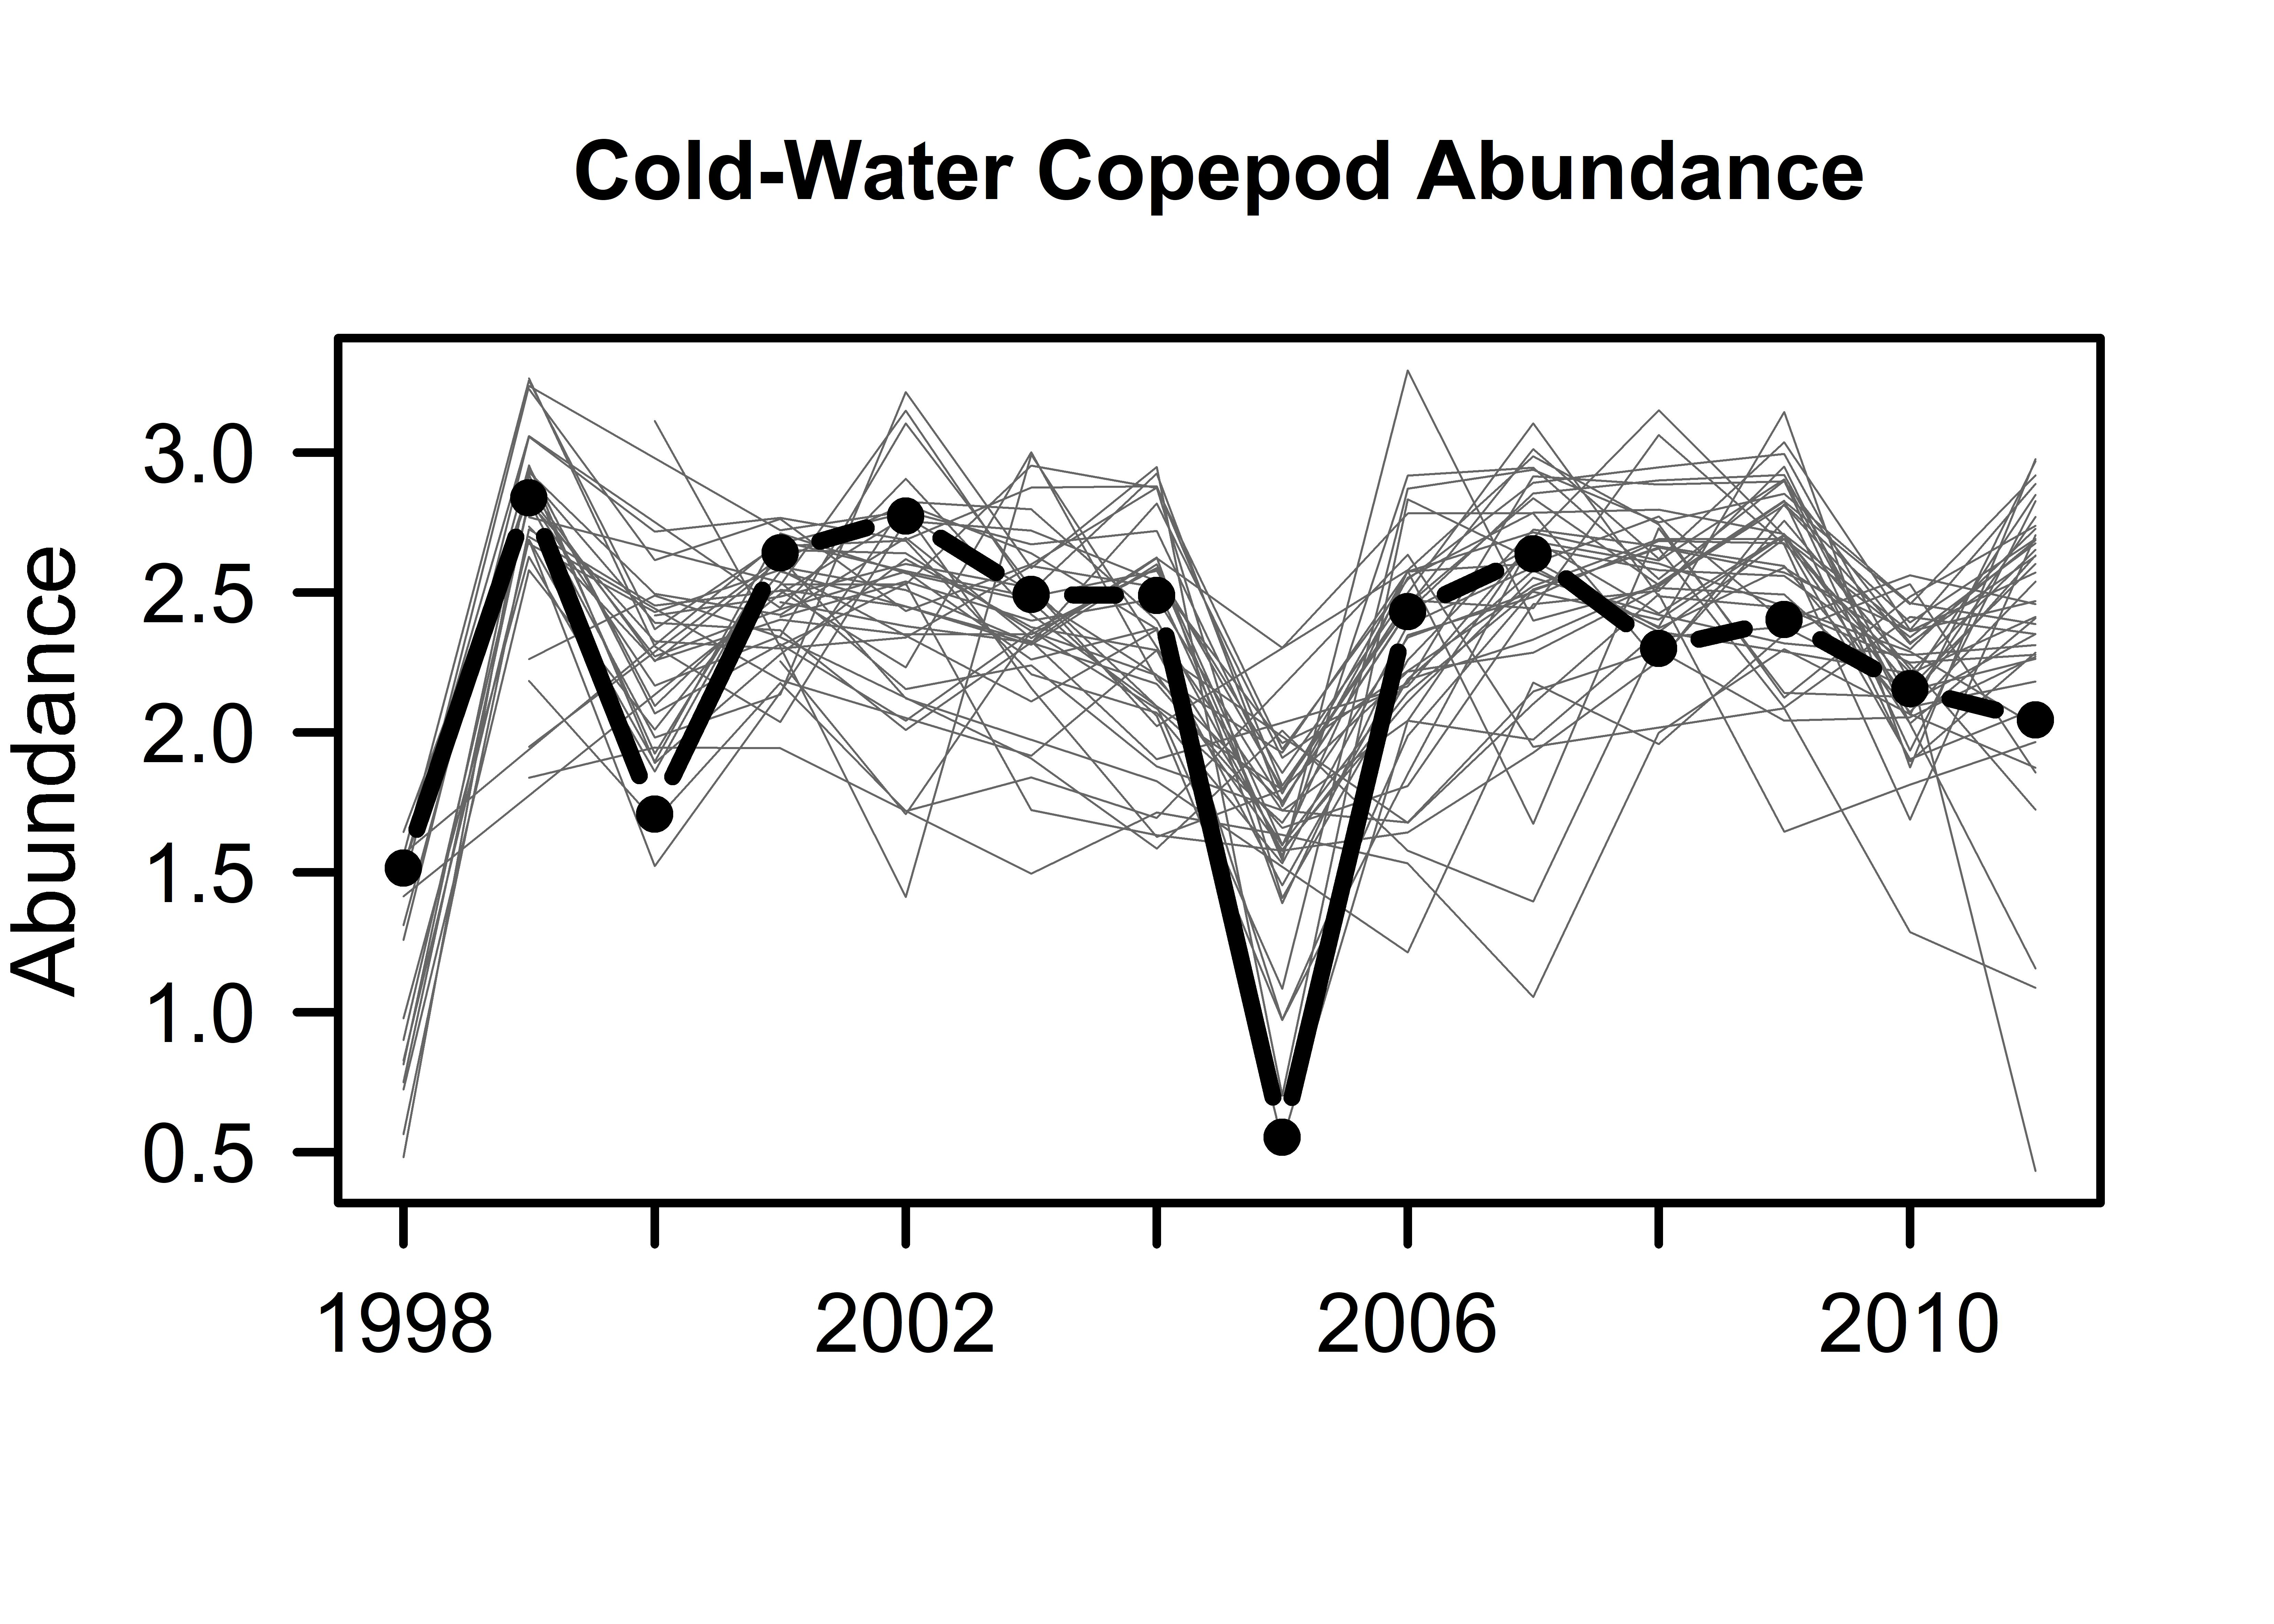
\includegraphics[width = 1\linewidth]{images/nor_abu.jpg}
  \caption{}
  \label{fig:cold_abu}
\end{subfigure}
\begin{subfigure}{0.45\textwidth}
  \centering
  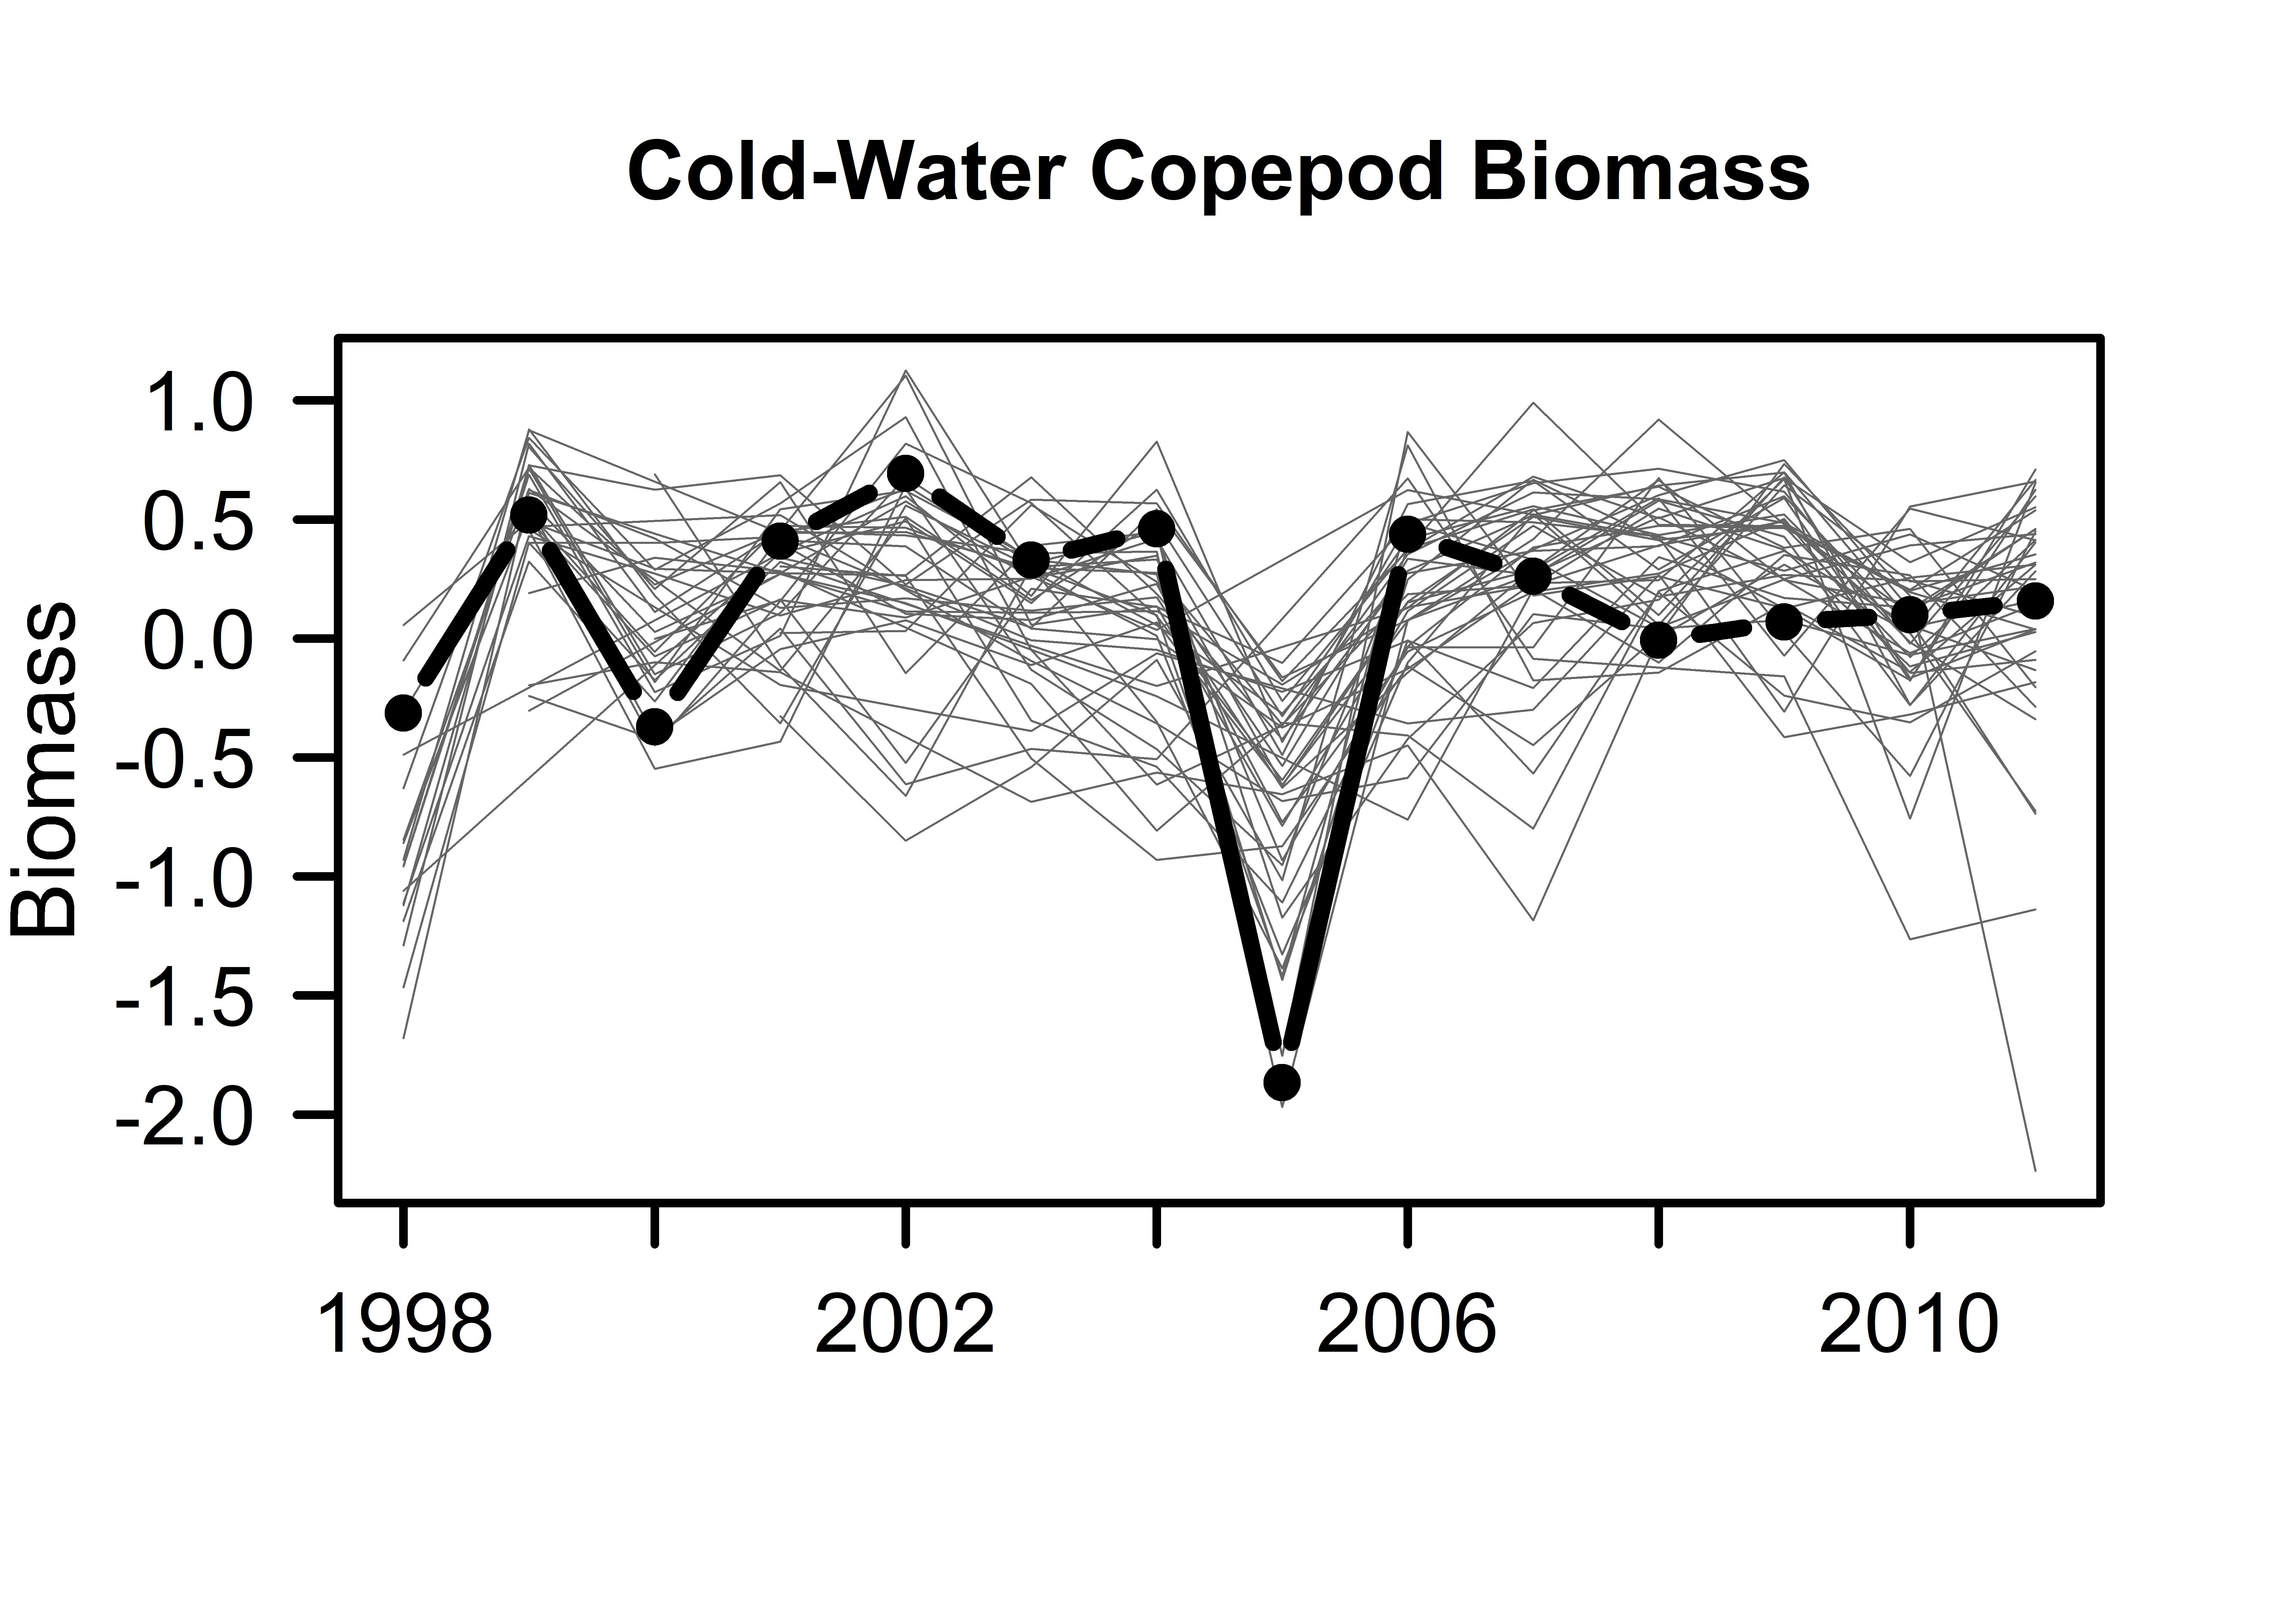
\includegraphics[width = 1\linewidth]{images/nor_bio.jpg}
  \caption{}
  \label{fig:cold_bio}
\end{subfigure} \\
\begin{subfigure}{0.45\textwidth}
  \centering
  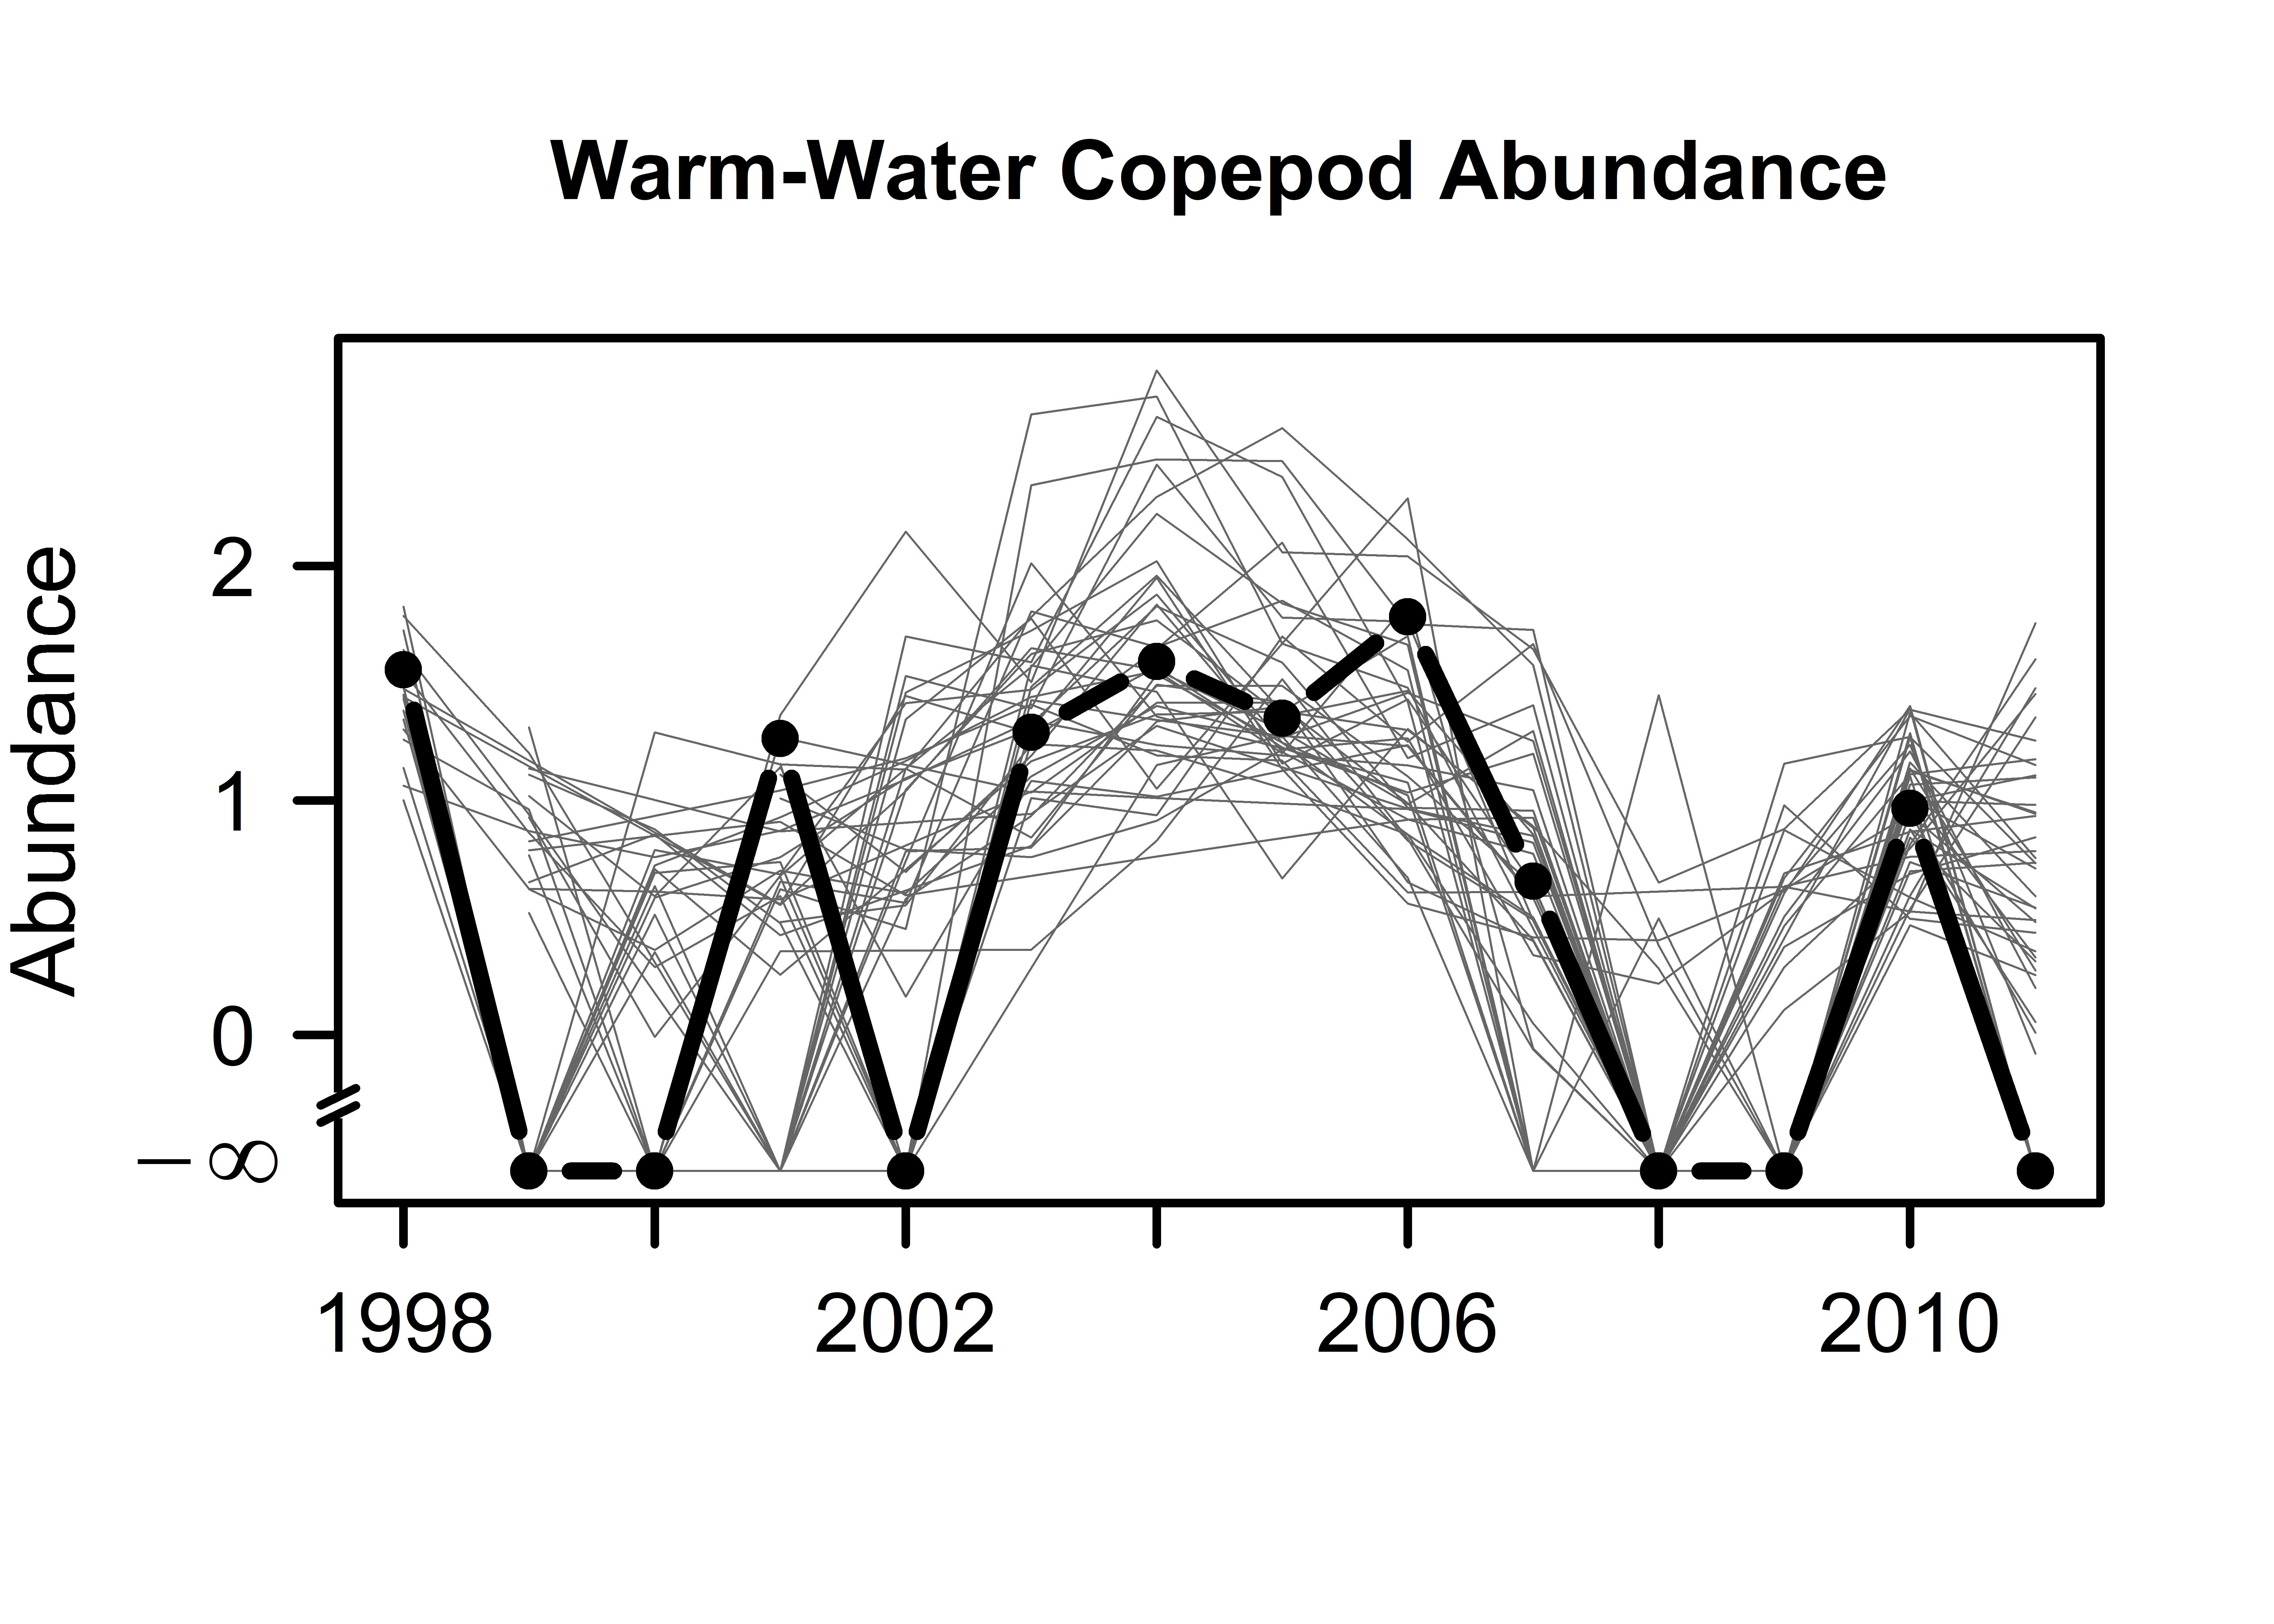
\includegraphics[width = 1\linewidth]{images/so_abu.jpg}
  \caption{}
  \label{fig:warm_abu}
\end{subfigure}
\begin{subfigure}{0.45\textwidth}
  \centering
  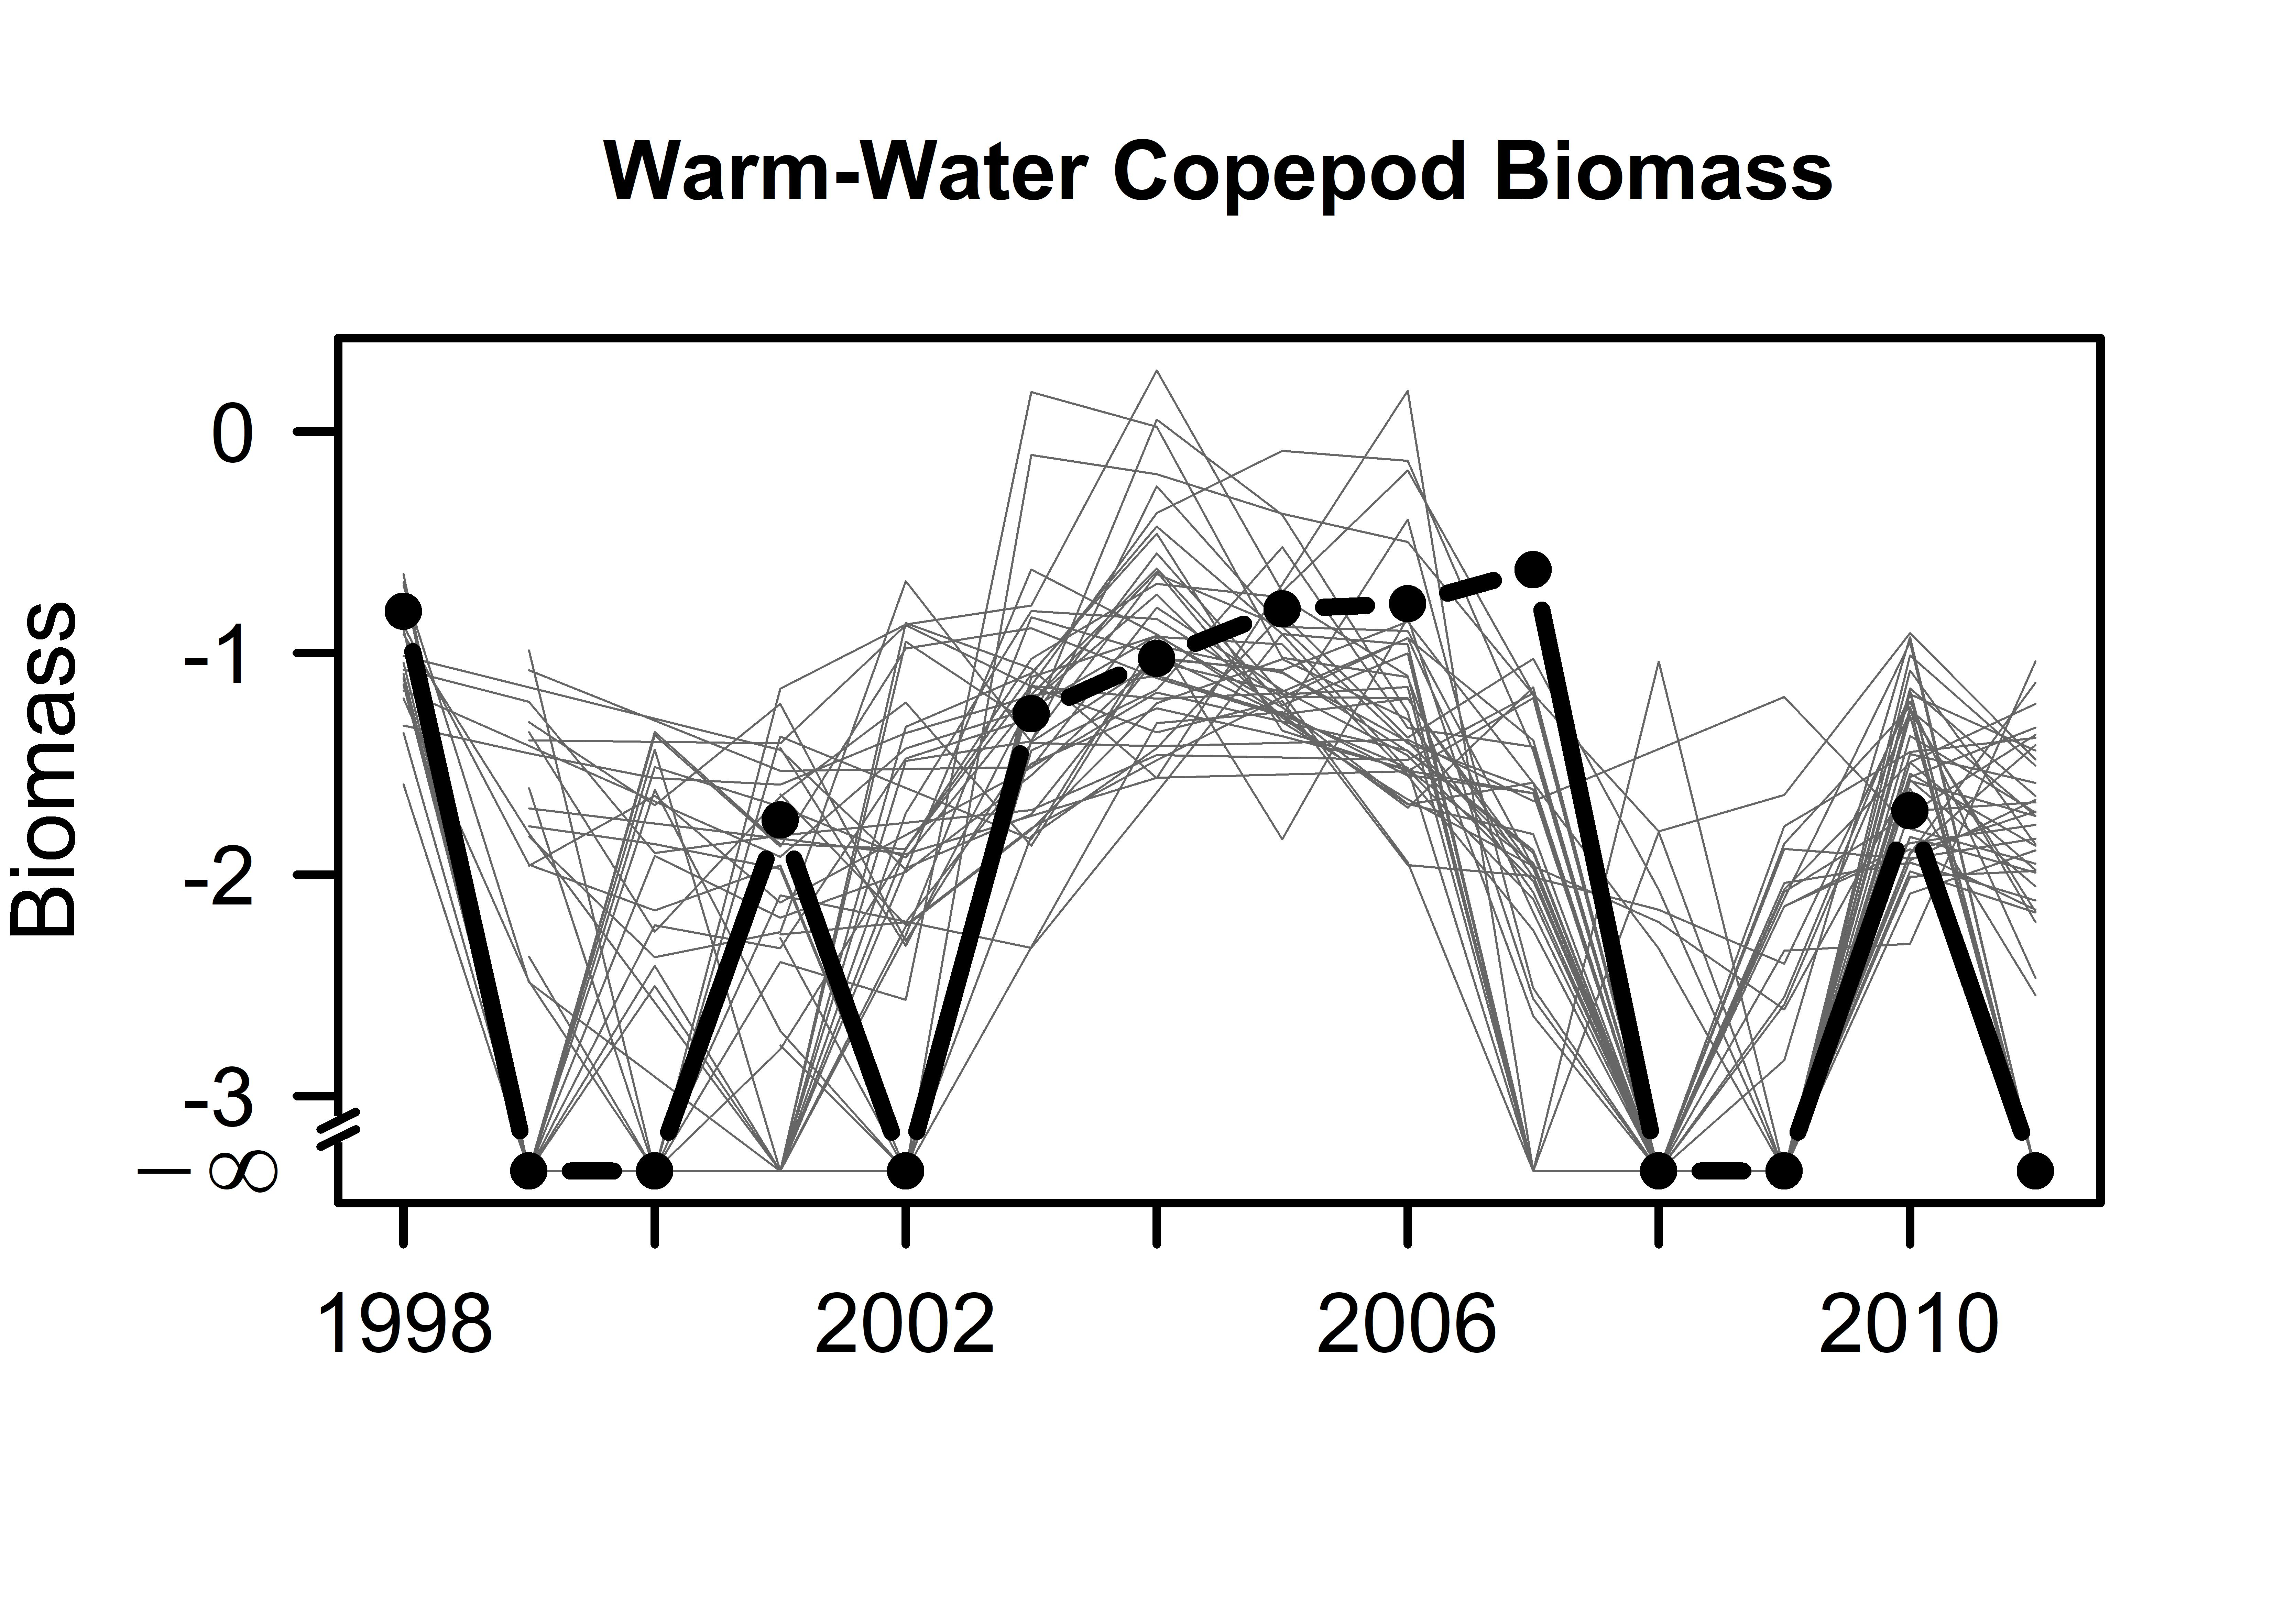
\includegraphics[width = 1\linewidth]{images/so_bio.jpg}
  \caption{}
  \label{fig:warm_bio}
\end{subfigure}
\caption{Time series of cold-water copepod abundance (top-left), cold-water copepod biomass (top-right), warm-water copepod abundance (bottom-left), and warm-water copepod biomass (bottom-right) $\log_{10}$ averages. Average $\log_{10}$ abundance or $\log_{10}$ biomass at NH05 is indicated by the thick, black line with circles representing each individual year's average. Average $\log_{10}$ abundance or $\log_{10}$ biomass at all other stations are indicated by grey lines. Copepod abundance or biomass averages of zero are given a value of $-\infty$ after the $\log_{10}$ transformation, and this discontinuity is indicated by backslashes on the vertical axis of each plot.}
\label{fig:cope_ts}
\end{figure}

The metric-taxa-station-year combinations were used to compute Spearman correlations between NH05 and all other stations. Spearman correlations were preferred to Pearson correlations for two reasons. First, Spearman correlations are rank based, which means they are less sensitive than Pearson correlations to particularly anomalous years. Second, Spearman correlations, unlike Pearson correlations, are not hindered by a restrictive linearity assumption.

To compute the Spearman correlation between two stations, the metric-taxa-station-year combinations must share a metric-taxa-year identifier. For example, if $\mathbf{x}$ denotes the abundance-warm-NH05 correlations, and $\mathbf{y}$ denotes the abundance-warm-NH15 correlations, then the pair ($\mathbf{x}_{1998}, \mathbf{y}_{1998}$) represents these metric-taxa-station combinations during 1998. The observations are paired for each year and the correlation is computed using these pairs. Between station correlations are so useful because they help us use patterns at NH05 to inform patterns at other stations. For example, if the abundance of warm-water copepods at NH05 and the abundance of warm-water copepods at NH15 are highly correlated, then an above average abundance year at NH05 should imply an above average abundance year at NH15.  The number of pairs available to compute correlations equals the number of metric-taxa-year identifiers each station shares (Table \ref{tab:station_sampling}). For example, NH05 was sampled all 14 years during 1998-2011, but NH20 was only sampled during 12 of those years -- NH20 was not sampled during 1999 or 2000. Thus, only the 12 available pairs are used to compute correlations involving NH05 and NH20.

We computed correlations between NH05 and all other stations sampled at least 10 of the 14 years during 1998-2011. The more stations NH05 is highly correlated with, the more representative NH05 is of patterns in the NCC, and hence, the more effective NH05 is as a sentinel station regarding these response metrics. Of the 55 stations sampled at least once during 1998-2011 (Figure \ref{fig:station_layout}), 42 stations were sampled at least 10 years. One of these stations was NH05, so in total, there were 41 stations available to compute correlations with NH05. NH05 correlations were estimated separately for each metric-taxa combination: abundance-warm, biomass-warm, abundance-cold, biomass-cold. Though the correlation estimate gives an idea of the dependence relationship between two stations, it is important to quantify the uncertainty in this estimate using a statistical hypothesis test. The p-values from this statistical hypothesis test were computed and used to evaluate the likelihood the observed correlation estimate occurred due to random chance.  Within each metric-taxa combination, p-values were adjusted using the Benjamini-Hochberg approach to control for multiple comparisons \citep{benjamini1995controlling}.

Though our primary focus was to quantify the cold-water and warm-water copepod correlations between NH05 and other stations in the NCC, we explored two additional extensions.  First, we computed correlations between NH05 and all other stations in the NCC for several metric-species combinations, where the species evaluated are from Table \ref{tab:copepod_table}. Second, we treated each station in the NCC sampled at least 10 years as a sentinel station and evaluated its performance with respect to abundance and biomass. This analysis was used to identify stations that are most representative of the NCC's broad patterns, and hence, the most effective sentinel stations. For every station, each metric-taxa combination has 41 correlation estimates. An average of these station’s estimates weighted by the sample sizes yields a single summary at that station for that metric-taxa combination.  For example, consider the weighted average of all 41 warm-water abundance correlations between NH05 and the other stations. The larger this weighted average, the more representative NH05 is of the warm-water copepods. These weighted averages were computed for each station and used to easily identify the most representative stations in the NCC. This multiple sentinel station approach was also repeated for each metric-species combination. To perform all analyses, the software language R \citep{rcore2019r} and the R package \textit{pairedstats} \citep{dumelle2021pairedstats} were used. 

\section{Results}

\subsection{NH05 Correlations}\label{subsec:nh05_cors}


\begin{figure}
  \centering
  \includegraphics[width = .75\textwidth]{images/warm_nh05.tif}
  \caption{Warm-water abundance and biomass correlations (left) and adjusted p-values (right) with NH05.  Circles are offset to prevent overlapping. The 50, 100, 150, and 200m depth contours are indicated by dotted lines.  NH05 is indicated by an X. }
  \label{fig:warm_nh05}
  \includegraphics[width = .75\textwidth]{images/cold_nh05.tif}
  \caption{Cold-water abundance and biomass correlations (left) and adjusted p-values (right) with NH05.  Circles are offset to prevent overlapping. The 50, 100, 150, and 200m depth contours are indicated by dotted lines.  NH05 is indicated by an X. }
  \label{fig:cold_nh05}
\end{figure}

For each metric-taxa combination, nearly all correlation estimates between NH05 and other stations were positive (Figure \ref{fig:warm_nh05} and Figure \ref{fig:cold_nh05}). These positive correlation estimates imply that larger abundance or biomass values at NH05 were associated with larger abundance or biomass values at the other stations. Correlation estimates for the warm-water copepods tended to be much larger than correlation estimates for the cold-water copepods (Figure \ref{fig:warm_nh05} and Figure \ref{fig:cold_nh05}).  Within each copepod taxa, abundance correlation estimates tended to be larger than biomass correlation estimates (Figure \ref{fig:warm_nh05} and Figure \ref{fig:cold_nh05}). For the four metric-taxa combinations, the average NH05 correlation estimates were 0.66 (abundance-warm), 0.55 (biomass-warm), 0.44 (abundance-cold) and 0.27 (biomass-cold). For the warm-water copepods, there were several small p-values associated with the correlation estimates: 82.9\% (abundance) and 63.4\% (biomass) of stations had correlations whose adjusted p-values were less than 0.1 (Figure \ref{fig:warm_nh05} and Table \ref{tab:warmcold_nh05}).
\begin{table}
    \footnotesize
    \centering
    \begin{tabular}{llcccc}
    \hline
    \hline
          & & \multicolumn{2}{c}{Adj. p $< 0.05$} & \multicolumn{2}{c}{Adj. p $< 0.10$} \\
          Metric & Taxa & Stations & Cor. Est & \% Stations & Cor. Est \\
         \hline
         Abundance & Warm-water  & 61.0\% &  (0.63, 0.89) & 82.9\% & (0.53, 0.89) \\
         Biomass & Warm-water  & 36.6\% & (0.68, 0.85) & 63.4\% & (0.53, 0.85) \\
         Abundance & Cold-water & 12.1\% &  (0.71, 0.87) & 36.6\% & (0.58, 0.87) \\
         Biomass & Cold-water & 0.0\% & (NA, NA) & 0.0 \% & (NA, NA) \\
         \hline
    \end{tabular}
    \caption{Correlation estimates and p-values for abundance and biomass of warm-water and cold-water taxa. For each adjusted p-value category (Adj. P), two quantities are presented: the percentage of stations (\% Stations) whose correlation estimates have adjusted p-values in the respective category, and the range of correlation estimates (Cor. Est) in the respective category.}
    \label{tab:warmcold_nh05}
\end{table}
But for cold-water copepods, these p-values were much larger: 36.6\% (abundance) and 0.0\% (biomass) of stations had correlations whose adjusted p-values were less than 0.1 (Figure \ref{fig:cold_nh05} and Table \ref{tab:warmcold_nh05}).
For all metric-taxa combinations, correlations estimates with NH05 tended to be higher at midshelf stations and lower at stations closest to shore or stations past the shelf break. Station depths are provided in Table \ref{tab:station_sampling}. 

We also analyzed correlations with NH05 for all metric-species combinations. While further details regarding the metric-species analyses are provided in Appendix \hyperlink{appendixB}{B}, here we provide a few important results. \textit{Paracalanus parvus} had the highest average correlations among the warm-water species (abundance: 0.82, biomass: 0.84). For both abundance and biomass, 100.0\% of \textit{Paracalanus parvus} correlations had adjusted p-values less than 0.1 (Figure \ref{fig:PP_nh05}). In contrast, \textit{Calanus pacificus} had much lower average correlations (abundance: 0.50, biomass: 0.51). 9.8\% (abundance) and 41.4\% (biomass) of \textit{Calanus pacificus} correlations had adjusted p-values less than 0.1 (Figure \ref{fig:CP_nh05}).  \textit{Acartia longiremis} had the highest average correlations among the cold-water species (abundance: 0.43, biomass: 0.52). 34.1\% (abundance) and 51.2\% (biomass) of \textit{Acartia longiremis} correlations had adjusted p-values less than 0.1 (Figure \ref{fig:AL_nh05}). \textit{Pseudocalanus} spp. had the lowest correlations of the cold-water copepods (abundance: 0.32, biomass: 0.27). 2.4\% (abundance) and 0.0\% (biomass) of \textit{Pseudocalanus} spp. correlations had adjusted p-values less than 0.1 (Figure \ref{fig:PC_nh05}).  

\subsection{The Utility of Other Sentinel Stations}

In Section \ref{subsec:nh05_cors}, we evaluated the representativeness of NH05 with respect to cold-water and warm-water copepods. We repeated this process for each individual station to determine which are most representative of the entire region, i.e. the most effective sentinels. The average correlation estimate across all stations was much higher for the warm-water copepods (abundance: 0.59, biomass: 0.58) than the cold-water copepods (abundance: 0.38, biomass: 0.34), as seen in Figures \ref{fig:coldwarm_all} and \ref{fig:coldwarm_depth}.
\begin{figure}
\centering
  \includegraphics[width = .75\textwidth]{images/coldwarm_all.tif}
  \caption{Cold-water (left) and warm-water (right) abundance and biomass average correlations evaluating the utility of each station as a sentinel.  Negative correlations are not given colors and instead represented by white filled circles.  The 50, 100, 150, and 200m depth contours are indicated by dotted lines.}
  \label{fig:coldwarm_all}
    \includegraphics[width = .75\textwidth]{images/coldwarm_depth.TIF}
  \caption{Warm-water and cold-water abundance and biomass average correlations. The average correlation for each station is viewed as a function of depth.}
  \label{fig:coldwarm_depth}
\end{figure}
The patterns of the average correlation estimates for each station as a function of depth are seen in Figure \ref{fig:coldwarm_depth}. For the warm-water copepods, there does not seem to be a strong relationship between depth and the average correlation estimate.  But for cold-water copepods, there is a quadratic relationship: average correlation estimates increase from 0 m, peak near 100 m, and then begin to decrease again. We performed the same type of analysis for each metric-species combination, and these results are summarized in Appendix \hyperlink{appendixC}{C}; one important finding was that across all stations, \textit{Paracalanus parvus} had the highest average correlations (abundance: 0.79, biomass: 0.79) among the warm-water copepods, and \textit{Acartia longiremis} has the highest average correlations (abundance: 0.42, biomass: 0.49) among the cold-water copepods.

We also ranked each station by its average correlation estimate within the four metric-taxa combinations. The highest ranks are provided in Appendix \hyperlink{appendixD}{D}, but four important results are summarized next.  First, NH05’s had rankings near the middle for all four metric-taxa combinations. Second, QR19 had the best performance for both warm-water abundance and warm-water biomass.  Third, GH21 had the best performance for both cold-water abundance and cold-water biomass.  Fourth, NH15 had the highest average ranking across the four metric-taxa combinations, followed closely by WB05.  

\section{Discussion}

We found that throughout the study region, NH05 was a more representative sentinel station for the warm-water copepod community than the cold-water copepod community, with abundance at NH05 tending to be slightly more representative than biomass.  In our analysis of treating every station as a sentinel, warm-water copepods again had higher correlations throughout the region than cold-water copepods.  For the cold-water copepods, the highest correlations were found at mid-shelf stations.  These results are reflective of differences in latitudinal and cross-shelf oceanographic processes, timing and strength of local upwelling, and basin-scale processes that influence the copepod community.   

\subsection{Warm-Water Copepods}

When warm-water copepods were prevalent off central Oregon in June, they were almost uniformly present in low numbers throughout the region during warm ocean conditions and almost absent during years that exhibited cool ocean conditions. Warm-water copepods were nearly absent across all stations during anomalously cool ocean conditions in 2008 and 2009, and they were absent on the inner-mid shelf during other years that were not anomalously warm (Table \ref{tab:station_sampling}). Their absence on the inner-mid shelf was likely due to advective processes associated with upwelling.   Warm-water copepods are generally present off Oregon during the winter and periods of downwelling when less advective processes and more consistent hydrographic conditions exist across the shelf \citep{keister2003zonal, keister2011zooplankton}. These taxa are noted for having relatively low abundance, low biomass, and a high species richness as compared to the cold-water copepods that are more common during spring and summer \citep{peterson1977seasonal}.  


Warm-water copepods can also be found off the Oregon and Washington shelf in summer during warm phases of the PDO, during El Niño events, and when upwelling is delayed or weak. Our study spanned multiple climatic events that led to anomalously warm ocean conditions throughout the NCC.  The study occurred when the PDO was in positive phase for multiple years (1998, 2003-2007, 2010), during five El Niño events (1997-98, 2002-03, 2004-05, 2006-07, 2009-10), and one of these years, 2005, had delayed upwelling. When the PDO is in positive phase, the strength of the Aleutian Low increases, which results in reduced equatorward wind stress and increased onshore and poleward flow throughout the NCC \citep{mantua1997pacific}. Poleward flow can also occur during El Niño events from the northward propagation of coastally trapped waves and from local atmospheric forcing that reduces upwelling-generating alongshore winds \citep{hermann2009comparison, di2013double, frischknecht2017local}. During 2005, the lack of strong northerly winds delayed upwelling until late September that year, allowing stratified ocean conditions to develop and persist \citep{kosro2006physical}. These climatic events result in poleward and onshore flow that reduces cross-shelf and alongshore gradients and leads to increased stratification and reduced productivity over large spatial scales. During all of the events described above, warm-water copepods also dominate the copepod community on the central Oregon shelf \citep{keister2011zooplankton, fisher2015impact}. 

Overall, warm oceanographic conditions promote a widespread low abundance and highly diverse warm-water copepod community throughout the NCC during summer. These patterns, in concert with the near absence of warm water copepods during anomalously cool ocean conditions, drove the strong spatial coherence of warm-water copepods across stations throughout our study region.  As a result, a multitude of stations, including NH05 could be used as sentinel stations for our sampling region during warm oceanographic conditions.  When all stations were treated as a sentinel, however, four out of five stations with the highest warm-water correlations were on the Washington shelf; QR19 had the highest average correlation and NH15 was the only station from the Oregon shelf (Table \ref{tab:warmcold_rank}). This is most likely due to less wind-driven advection and retentive qualities of the Washington shelf.

\subsection{Cold-Water Copepods}

Unlike the warm-water copepods having high correlations between NH05 and the other stations in the NCC, for the cold-water copepods, there were few stations whose correlations with NH05 had small adjusted p-values, especially for biomass. This can partly be explained by the highly advective and dynamic features of upwelling systems.  Cold-water copepods dominate the Oregon and Washington shelf during summer when wind driven upwelling drives equatorward transport that delivers cold-water copepods to the shelf. Upwelled waters also transport nutrients into the euphotic zone, triggering blooms of phytoplankton that can sustain zooplankton populations \citep{bograd2009phenology}. Variability in alongshore wind stress and topographically generated mesoscale features lead to latitudinal clines in upwelling strength across the region, while event scale wind stress increases cross-shelf variability by modifying the location of the upwelling jet on finer spatial scales \citep{castelao2005coastal}. On inter-annual time scales, basin-scale processes can also modify alongshore flow and wind stress that can affect the abundance and distribution of cold-water copepods. The combination of differing nutrient sources, weaker wind-driven offshore advection, and a wide shelf increases phytoplankton bloom potential and retention, which could also result in the retention of zooplankton. 

Off the Oregon coast, the shelf is narrow and wind stress is strong, yet upwelling winds are sustained for a number of days, followed by a relaxation period creating rapid changes in the hydrography. These upwelling relaxation cycles greatly influence the distribution of cold-water copepods on the shelf.  For example, the process of upwelling creates advective currents (both cross-shelf and alongshore) moving water masses and their zooplankton south and off the shelf, and therefore, out of our sampling region.  The strength of these advective currents varies by depth (strongest near the surface) and proximity to shore (typically strongest near the coast but dependent on bottom topography).  All factors listed above underscore the patchy, highly variable aggregations of cold-water copepods, with potentially exponential differences in abundance and biomass both temporally and spatially during the summer \citep{peterson1977seasonal}. Therefore, the lack of significant correlations of NH05 with many stations for the cold-water copepods could be primarily due to its location in the most southern range of the sampling grid, which makes it one of the most susceptible to upwelling conditions which are stronger, more persistent, and therefore more advective than many of the other sampled stations.  When every station was treated as a sentinel, cold-water copepod correlation values at many stations off the Washington shelf also did not perform exceptionally better than the stations located on the Oregon shelf. When ranked, the best performing stations were located off of both the central Washington to northern Oregon (Gray's Harbor and Cape Meares transects) (Table \ref{tab:warmcold_rank}).

Unlike the warm-water copepods that are present in the NCC in the summer during warm ocean conditions, cold-water copepods are present regardless of ocean conditions, with the exception of extreme events such as the 1997-98 El Ni{\~n}o and the marine heatwave in 2014-16, when they were absent \citep{fisher2015impact, peterson2017pelagic}. Therefore, the underlying variability in abundance and biomass combined with a ‘snapshot in time’ sampling suggests that we should not expect strong correlations with the cold-water copepods throughout the region, especially when sampling spans both large scale climatic events and localized synoptic wind events. Future analysis warrants investigating whether the distribution of cold-water copepod correlations are more homogeneous during similar ocean conditions and whether biomass and abundance are more strongly correlated with more southern locations.

\subsection{Cross-Shelf Variability: Mid-Shelf Correlations}

The advective effects of upwelling during cold-water conditions most likely drove the quadratic pattern observed between correlation values for the cold-water copepods and depth, where the highest values were found at stations between 50–150 m (Figure \ref{fig:coldwarm_depth}). Several studies have previously documented cross-shelf zonation of copepod taxa off Oregon \citep{peterson1979zonation, keister2003zonal, morgan2003onshore} and Washington \citep{landry1989broad}, identifying taxa typical of nearshore waters (depths less than approximately 50 m), shelf waters, and offshore (greater than 180 m depth).   Our three cold-water taxa are typical of shelf-waters during upwelling and cold summers whereas the warm-water group includes the offshore taxa that are found only on the shelf in summer during warm climatic events.  Upwelling driven advection is strongest on the mid-shelf approximately 10-15 km from shore. Inshore of the upwelling front, circulation is generally alongshore, while offshore advection decreases moving westward of the upwelling front, only influencing the offshore copepod communities during strong persistent upwelling conditions \citep{peterson1979zonation}.   NH03, a station located 5.5 km from shore (only two nautical miles inshore of NH05) and inshore of the upwelling front, had the third to lowest ranking of correlation values compared to all other stations in our study. This is likely due to the alongshore circulation inshore of the upwelling front that has little mixing with mid-shelf to offshore waters.  The same relationship between correlation values with depth was not seen with the warm-water copepods. Warm-water oceanographic conditions, which result in warm-water copepods on the shelf, are typically either stratified waters or downwelling, where water masses are driven from both the south and west onto the shelf shoreward with greatly reduced cross-shelf gradients.  Neither of these conditions create the types of variability in the copepod population found in upwelling favorable conditions, allowing both higher correlations and spatial uniformity in these correlations for the warm-water copepods.  Interestingly, when treating all stations as a sentinel, the mid-shelf station NH15 performed best overall over both cold and warm years, most likely due to the aforementioned factors.  

\subsection{NH05 Abundance and Biomass Correlation Discrepancies}

When comparing NH05 to all other stations, our abundance correlations were generally higher than biomass correlations, regardless of water mass affinity.  This is unsurprising considering the fact that NH05 is both physically and biologically dynamic when compared to all other stations in our study.  Generally speaking, abundance can be very similar even with different proportions of species between stations, whereas comparisons of biomass between the same stations are much more species dependent.  Variability in biomass between multiple species in our study is potentially very high.  For example, the mean dry weight Carbon per female for \textit{Acartia longiremis} is 6 $\mu$g \citep{uye1982length} versus 109 $\mu$g for a female \textit{Calanus marshallae} \citep{peterson1980life}.  Therefore, it would take over eighteen \textit{Acartia longiremis} to equal the dry weight Carbon of one \textit{Calanus marshallae}.  These differences in individual species biomass potentially create an exponentially broader range in values compared with abundance alone and therefore influence lower correlation values  for biomass. The other aspect of copepod life history that would also account for station to station differences in abundance versus biomass is the proportion of the six copepod life history stages that were sampled.  Higher proportions of later stages, especially for a larger copepod such as \textit{Calanus marshallae}, would contribute significantly more to a stations total biomass than lower stages.  

\subsection{Species-Specific Findings}


Within our analysis, two species (one from each copepod group) had higher individual correlations than all the others did in their respective groups: the warm-water species \textit{Paracalanus parvus}, and the cold-water species \textit{Acartia longiremis}.  Both species are considered on-shelf species but have been found at a wide range of depths from shallow to offshore stations during their respective basin-scale climatological events \citep{peterson2002effect, keister2003zonal}. This combination of ubiquity in sample presence and consistent abundance reflecting either warm (\textit{Paracalanus parvus}) or cold (\textit{Acartia longiremis}) conditions suggests they are both more representative of regional trends than any other species in our study.  Thus a lack of spatial coherence in correlations of the other two individual cold-water taxa, \textit{Calanus marshallae} and \textit{Pseudocalanus} spp., clearly influenced the low correlations for all stations throughout the region with respect to the cold-water taxa group.  For the warm-water copepod group, several other taxa provided relatively high correlations, in addition to \textit{Paracalanus parvus}, providing higher correlations among the region for the entire group. 


\section{Conclusions}

A driving goal of William T. Peterson’s work was to document physical and biological conditions that could inform fisheries managers.  As introduced previously, due to high correlations with basin and regional scale processes, several metrics of the copepod community at NH05 (e.g. anomalies of biomass of cold and warm-water copepod groups and species richness, the date of the spring biological transition) have become key components of ecosystem status reports \citep{wells2017state, harvey2018ecosystem, harvey2019ecosystem, thompson2018state, thompson2019state}. Peterson’s initial intent in 2005 to display these indicators, as well as multiple physical indicators such as mean SST, in a red-light, green-light ‘stop-light chart’ as a qualitative summary of “good” and “poor” ocean conditions for stakeholders and managers of juvenile salmon came to fruition (see \href{https://www.nwfsc.noaa.gov/oceanconditions}{https://www.nwfsc.noaa.gov/oceanconditions}). The copepod metrics from NH05 have been used in several statistical models of salmon ocean performance \citep{burke2013multivariate, peterson2014applied, tucker2015coastal} and operational models of salmon survival and adult return abundance \citep{rupp2012marine, zimmerman20122010}. In general, the NH Line is highlighted as an important example of research and monitoring efforts valuable for ecosystem–based management, having the longest consistent oceanographic sampling program in the NCC between southern California to British Columbia \citep{harvey2020importance}.

The copepod indices of warm-water and cold-water copepod biomass from NH05 are useful ecosystem indicators as they capture the inter-annual variability in ocean conditions and forage that affect juvenile salmon survival. As our results indicate, however, on finer spatial scales, the copepod communities sampled at NH05 do not, and are not expected to, correlate highly with every other station across the Oregon and Washington shelf.  By their very nature plankton are patchy and high variability temporally and spatially in plankton distributions and abundances have been well documented, even along the Oregon coast \citep{peterson1979zonation, peterson2002effect, keister2003zonal, morgan2003onshore}. Each copepod species has unique life history traits and behavioral responses at different ontogenic stages affecting their general spatial distribution under variable ocean conditions \citep{peterson1979zonation}.

Despite this unavoidable oceanographic variability and patchiness of plankton, when every station was treated as a sentinel, our analysis found that even under upwelling and potentially highly advective conditions, cold-water copepod correlations were higher at mid-shelf stations such as GH21, which had the highest correlations among cold-water copepods (Table \ref{tab:warmcold_rank}). Whereas NH05 is at the shallow side of mid-shelf (at a depth around 60 m), NH15, which is at a depth around 89 meters, had the highest overall correlations (Table \ref{tab:all_rank}).  Although no one station ranked highest for all categories, it is possible that NH15 would more closely reflect conditions on a finer spatial scale throughout the Oregon-Washington shelf. After NH15, WB05 off Washington had the second highest average ranks across all categories. Our results suggest NH15 and WB05 may be fairly representative of the NCC region regardless of response metric (abundance or biomass) or copepod taxa (warm-water or cold-water). It is also important to note, however, that this study was conducted with data collected only in June, and different sampling periods may have given different results. The strength of the NH05 indicators are the high frequency (twice monthly), year round sampling that captures inter- and intra-annual variability in the bioenergetics of the food chain and that it is a location that is easily accessible all year.

In conclusion, most stations had similar correlations for warm-water copepods and NH05 generally did as well as any other station as a sentinel of ecosystem indicators during the conditions which promote their relatively equal distribution throughout the NCC. The contrasting result of lower correlations for nearly all stations for cold-water copepods provides evidence for higher spatial variability during conditions that transport cold-water into the NCC. Thus, our findings do not dispute that NH05 is an appropriate sentinel for regional and basin scale oceanographic events. It is no surprise, however, that our understanding of fine scale dynamics in the NCC could benefit from additional finer scale sampling, both spatially and temporally. 

%%%%%%%%%%%%%%%%%%%%%%%%%%%%%%%%%%%%%%%%%%%%%%%%%%%%%%%
%%%%%%%%%%%%%%%%%%%%%%%%%%%%%%%%%%%%%%%%%%%%%%%%%%%%%%
%   Supplementary Material
%%%%%%%%%%%%%%%%%%%%%%%%%%%%%%%%%%%%%%%%%%%%%%%%%%%%%%
%%%%%%%%%%%%%%%%%%%%%%%%%%%%%%%%%%%%%%%%%%%%%%%%%%%%%%

 






\section{Declarations of Interest:}
none.

\section{Funding:}
Funding for this study was provided by the Bonneville Power Administration (Project 1998-014-00) and the Northwest Fisheries Science Center, National Marine Fisheries Service, National Oceanic and Atmospheric Administration.

\section{Acknowledgments}
This paper is dedicated to Dr. William T. Peterson. Without his passion and dedication, none of this work would have been possible. His intellect, wit, good nature, and humor has influenced many people within the oceanography community, young and old. He had a true ability to take complex ecological concepts and translate them eloquently and often entertainingly to a wide audience. We miss him dearly as a colleague, mentor, and friend.

We greatly appreciate the many people who contributed to this project over the years,
including the captains and crews who operated vessels, especially the FV \textit{Frosti}, and the many scientists who helped collect the samples. Funding for this study was provided by the Bonneville Power Administration (Project 1998-014-00), Northwest Fisheries Science Center, National Marine Fisheries Service, and National Oceanic and Atmospheric Administration. We would like to thank Laurie Weitkamp, Dr. Eric Bjorkstedt, and three anonymous reviewers for constructive comments that greatly improved this manuscript.  We would also like to give a special thanks to Jennifer Fisher for the excellent feedback she provided throughout the writing of this manuscript.

\clearpage
\section*{Appendix A: Sampling Information}
\setcounter{table}{0}
\renewcommand{\thetable}{A.\arabic{table}}

The frequency of sampling at each station throughout the 1998-2011 Juvenile Salmon and Ocean Ecosystem Survey(JSOES) is provided in Table \ref{tab:station_sampling}.

% La Push
    {\scriptsize
    \begin{longtable}{llccccccccccccccr}
    \label{tab:station_sampling} \\
    \hline
    \hline
         Station & Depth (m) & 98 & 99 & 00 & 01 & 02 & 03 & 04 & 05 & 06 & 07 & 08 & 09 & 10 & 11 & Total   \\
         \hline
        LP04 & 34  & NA & C & C & C & C & CW & CW & CW & CW & CW & C & CW & CW & C & 13 \\
        LP06 & 50  & NA & CW & CW & CW & C & CW & CW & CW & CW & CW & C & C & CW & C & 13 \\
        LP09 & 78  & NA & C & CW & CW & CW & CW & CW & CW & CW & CW & CW & CW & CW & CW & 13 \\
        LP12 & 105 & NA & CW & C & CW & NA & CW & CW & CW & CW & CW & C & CW & CW & CW & 12 \\
        LP17 & 135 & NA & CW & C & CW & NA & CW & CW & CW & CW & CW & C & CW & CW & CW & 12 \\
        LP22 & 176 & NA & CW & CW & CW & NA & CW & CW & CW & CW & CW & C & C & CW & CW & 12 \\
        QR03 & 16  & NA & NA & NA & CW & C & CW & CW & CW & CW & CW & C & CW & CW & CW & 11 \\
        QR06 & 27  & NA & NA & NA & C & CW & CW & CW & CW & CW & C & C & C & CW & CW & 11 \\
        QR10 & 52  & NA & NA & NA & CW & C & CW & CW & CW & CW & CW & C & C & CW & CW & 11 \\
        QR14 & 77 & NA & NA & NA & CW & CW & CW & CW & CW & CW & CW & C & C & CW & CW & 11 \\
        QR19 & 112 & NA & NA & NA & C & CW & CW & CW & CW & CW & CW & C & C & CW & CW & 11 \\
        QR24 & 173 & NA & NA & NA & CW & CW & CW & CW & CW & CW & CW & CW & CW & CW & CW & 11 \\
        GH03 & 24  & NA & NA & C & CW & CW & CW & CW & CW & CW & CW & C & CW & CW & CW & 12 \\
        GH06 & 37  & NA & C & C & C & CW & CW & CW & CW & CW & CW & C & C & CW & C & 13 \\
        GH10 & 55  & CW & CW & C & C & CW & CW & CW & CW & CW & CW & C & C & CW & C & 13 \\
        GH16 & 81 & CW & C & CW & C & C & CW & CW & CW & CW & CW & CW & C & CW & CW & 14 \\
        GH21 & 111 & CW & CW & CW & CW & C & NA & CW & CW & CW & CW & C & CW & CW & CW & 13 \\
        GH26 & 150 & CW & CW & CW & CW & NA & CW & CW & NA & CW & CW & C & C & CW & CW & 12 \\
        GH31 & 155 & NA & CW & NA & CW & CW & NA & CW & NA & CW & CW & C & CW & CW & CW & 10 \\
        WB05 & 29  & CW & CW & NA & C & CW & CW & CW & CW & CW & C & C & C & CW & CW & 13 \\
        WB09 & 59  & CW & CW & NA & C & CW & CW & CW & CW & CW & CW & C & C & CW & CW & 13 \\
        WB14 & 80  & CW & NA & NA & CW & CW & CW & CW & CW & CW & CW & C & C & CW & CW & 12 \\
        WB19 & 109 & CW & NA & NA & CW & CW & CW & CW & CW & CW & CW & C & C & CW & CW & 12 \\
        WB23 & 128 & NA & NA & NA & CW & CW & CW & CW & CW & CW & CW & C & CW & CW & CW & 11 \\
        CR04 & 28  & NA & C & CW & CW & CW & CW & CW & CW & CW & CW & C & C & CW & CW & 13 \\
        CR07 & 55  & CW & C & C & CW & CW & CW & CW & CW & CW & C & C & CW & CW & C & 14 \\
        CR10 & 74  & CW & C & C & C & C & C & CW & CW & CW & C & CW & C & CW & CW & 14 \\
        CR15 & 110 & CW & C & CW & C & CW & CW & CW & CW & CW & C & C & C & CW & CW & 14 \\
        CR20 & 130 & CW & C & CW & CW & CW & CW & CW & CW & CW & CW & C & C & CW & CW & 14 \\
        CR25 & 150 & CW & C & CW & C & CW & CW & CW & CW & CW & CW & C & CW & CW & CW & 14 \\
        CR30 & 500 & NA & CW & CW & CW & CW & CW & CW &  & CW & CW &  & CW & CW & CW & 11 \\
        CM01 & 32  & NA & CW & C & CW & CW & CW & CW & CW & CW & CW & CW & CW & CW & CW & 13 \\
        CM03 & 56  & CW & C & CW & CW & CW & CW & CW & CW & CW & C & CW & C & CW & CW & 14 \\
        CM05 & 83  & CW & C & CW & CW & CW & CW & CW & CW & CW & CW & C & C & CW & C & 14 \\
        CM10 & 133 & NA & CW & CW & CW & CW & CW & CW & CW & CW & CW & C & CW & CW & CW & 13 \\
        CM15 & 174 & NA & CW & CW & CW & CW & CW & CW & CW & CW & CW & C & C & CW & CW & 13 \\
        CM20 & 245 & NA & CW & NA & CW & NA & CW & CW & NA & CW & CW & C & CW & CW & CW & 10 \\     
        NH03 & 44  & NA & NA & C & C & C & CW & CW & NA & CW & C & C & CW & CW & C & 11 \\
        NH05 & 58  & CW & C & C & CW & C & CW & CW & CW & CW & CW & C & C & CW & C & 14 \\
        NH10 & 78 & CW & C & CW & CW & C & CW & CW & CW & CW & C & C & C & CW & CW & 14 \\
        NH15 & 90 & CW & NA & NA & CW & CW & CW & CW & CW & CW & CW & C & C & CW & CW & 14 \\
        NH20 & 134 & NA & CW & NA & CW & CW & CW & CW & CW & CW & CW & C & C & CW & CW & 12 \\
    \hline
    \caption{Sampled JSOES stations. Stations sampled at least 10 times from June 1998 (98) to 2011 (11) where NA indicates the station was not sampled, C indicates only cold-water copepods were present, and CW indicates both cold-water and warm-water copepods were present. Transects have the following abbreviations: LaPush (LP), Queet's River (QR), Gray's Harbor (GH), Willapa Bay (WB), Columbia River (CR), Cape Meares (CM), Newport Hydrographic (NH).} % needs to go inside longtable environment
\end{longtable}}







\clearpage
\hypertarget{appendixB}{\section*{Appendix B: NH05 as a Sentinel}}
\renewcommand{\thesubsection}{B.1}
\setcounter{figure}{0} 
\renewcommand{\thefigure}{\small B.\arabic{figure}}
\setcounter{table}{0} 
\renewcommand{\thetable}{\small B.\arabic{table}}
\subsection{Warm-Water Species}

Summaries regarding the utility of NH05 as a sentinel station for metric-species combination are provided in Tables \ref{tab:warm_sp_nh05}. \textit{Calocalanus styliremis}, \textit{Calocalanus tenius}, and \textit{Mesocalanus tenuicornis} were not analyzed because they were either observed zero times (\textit{Calocalanus styliremis} and \textit{Calocalanus tenius}) or only once (\textit{Mesocalanus tenuicornis}). \textit{Paracalanus parvus} (Figure \ref{fig:PP_nh05}) and \textit{Acartia tonsa} have the highest NH05 correlations estimates. \textit{Calanus pacificus} (Figure \ref{fig:CP_nh05}), \textit{Clausocalanus} spp., \textit{Coryaeus anglicus}, and \textit{Ctenocalanus vanus} all had similar correlation estimates, but they were all much lower than the correlation estimates for \textit{Paracalanus parvus} and \textit{Acartia tonsa}. 
\begin{table}[ht]
    \footnotesize
    \centering
    \begin{tabular}{llrcrc}
    \hline
    \hline
           & & \multicolumn{2}{c}{Adj. p $< 0.05$} & \multicolumn{2}{c}{Adj. p $< 0.10$} \\
         Metric & Species  & \% Stations & Cor. Est & \% Stations & Cor. Est \\
         \hline
         Abundance & \textit{Acartia tonsa}  & 92.7\% &  (0.64, 1.00) & 97.6\% & (0.55, 1.00) \\
         Biomass & \textit{Acartia tonsa}  & 92.7\% &  (0.64, 1.00) & 97.6\% & (0.55, 1.00) \\
         Abundance & \textit{Calanus pacificus}  & 7.3\% &  (0.83, 0.93) & 9.8\% & (0.69, 1.00) \\
         Biomass & \textit{Calanus pacificus}  & 7.3\% &  (0.79, 0.87) & 41.5\% & (0.55, 0.87) \\
         Abundance & \textit{Clausocalanus} spp.  & 24.4\% &  (0.67, 0.91) & 31.7\% & (0.61, 0.91) \\
         Biomass & \textit{Clausocalanus} spp. & 17.1\% &  (0.69, 0.85) & 17.1\% & (0.69, 0.85) \\
         Abundance & \textit{Corycaeus anglicus}  & 36.6\% &  (0.63, 0.90) & 68.3\% & (0.51, 0.90) \\
         Biomass & \textit{Corycaeus anglicus}  & 24.4\% &  (0.71, 0.90) & 46.3\% & (0.57, 0.90) \\
         Abundance & \textit{Ctenocalanus vanus}  & 4.9\% &  (0.63, 1.00) & 68.3\% & (0.51, 1.00) \\
         Biomass & \textit{Ctenocalanus vanus}  & 12.2\% &  (0.69, 0.99) & 36.6\% & (0.55, 0.99) \\
         Abundance & \textit{Paracalanus parvus}  & 100.0\% &  (0.68, 0.91) & 100.0\% & (0.68, 0.91) \\
         Biomass & \textit{Paracalanus parvus}  & 100.0\% &  (0.63, 0.93) & 100.0\% & (0.63, 0.93) \\
         \hline
    \end{tabular}
    \caption{Correlation estimates and p-values of abundance and biomass of warm-water species. For each adjusted p-value category (Adj. P), two quantities are presented: the percentage of stations (\% Stations) whose correlation estimates have adjusted p-values in the respective category, and the range of correlation estimates (Cor. Est) in the respective category.}
    \label{tab:warm_sp_nh05}
\end{table}



%\captionsetup[subfigure]{labelformat = simple}
\begin{figure}[ht]
  \centering
  \includegraphics[width = 0.75\linewidth]{images/PP_nh05.tif}
  \caption{\textit{Paracalanus parvus} abundance and biomass correlations (left) and adjusted p-values with NH05 (right).  Circles are offset to prevent overlapping. The 50, 100, 150, and 200m depth contours are indicated by dotted lines.  NH05 is indicated by an X. }
  \label{fig:PP_nh05}
  \includegraphics[width = 0.75\linewidth]{images/CP_nh05.tif}
  \caption{\textit{Calanus pacificus} abundance and biomass correlations (left) and adjusted p-values with NH05 (right).  Circles are offset to prevent overlapping. The 50, 100, 150, and 200m depth contours are indicated by dotted lines.  NH05 is indicated by an X. }
  \label{fig:CP_nh05}
\end{figure}

\clearpage
\renewcommand{\thesubsection}{B.2}
\subsection{Cold-Water Species}

Summaries regarding the utility of NH05 as a sentinel station for metric-species combination are provided in Table \ref{tab:cold_sp_nh05}.  \textit{Acartia longiremis} (Figure \ref{fig:AL_nh05}) had the highest NH05 correlations estimates. \textit{Calanus marshallae} and \textit{Pseudocalanus} spp. (Figure \ref{fig:PC_nh05}) had similar correlation estimates, but they were both much lower than the correlation estimates for \textit{Acartia longiremis}.

\begin{table}[ht]
    \footnotesize
    \centering
    \begin{tabular}{llcccc}
    \hline
    \hline
          & & \multicolumn{2}{c}{Adj. p $< 0.05$} & \multicolumn{2}{c}{Adj. p $< 0.10$} \\
          Metric & Species & \% Stations & Cor. Est & \% Stations & Cor. Est \\
         \hline
         Abundance & \textit{Acartia longiremis} & 12.2\% &  (0.75, 0.81) & 34.1\% & (0.69, 0.82) \\
         Biomass & \textit{Acartia longiremis}  & 43.9\% &  (0.63, 0.92) & 51.2\% & (0.63, 0.92) \\
         Abundance & \textit{Calanus marshallae}  & 0.0\% &  (NA, NA) & 14.5\% & (0.66, 0.74) \\
         Biomass & \textit{Calanus marshallae}  & 0.0\% &  (NA, NA) & 0.0\% & (NA, NA) \\
         Abundance & \textit{Pseudocalanus} spp.  & 0.0\% &  (NA, NA) & 2.4\% & (0.80, 0.80) \\
         Biomass & \textit{Pseudocalanus} spp.  & 0.0\% &  (NA, NA) & 0.0\% & (NA, NA) \\
         \hline
    \end{tabular}
    \caption{Correlation estimates and p-values of abundance and biomass of cold-water species. For each adjusted p-value category (Adj. P), two quantities are presented: the percentage of stations (\% Stations) whose correlation estimates have adjusted p-values in the respective category, and the range of correlation estimates (Cor. Est) in the respective category.}
    \label{tab:cold_sp_nh05}
\end{table}


\begin{figure}[ht]
\centering
  \includegraphics[width = 0.75\linewidth]{images/AL_nh05.tif}
  \caption{\textit{Acartia longiremis} abundance and biomass correlations (left) and adjusted p-values with NH05 (right).  Circles are offset to prevent overlapping. The 50, 100, 150, and 200m depth contours are indicated by dotted lines.  NH05 is indicated by an X.}
  \label{fig:AL_nh05}
  \includegraphics[width = 0.75\linewidth]{images/PC_nh05.tif}
  \caption{\textit{Pseudocalanus} spp. abundance and biomass correlations (left) and adjusted p-values with NH05 (right).  Circles are offset to prevent overlapping. The 50, 100, 150, and 200m depth contours are indicated by dotted lines.  NH05 is indicated by an X.}
  \label{fig:PC_nh05}
\end{figure}











\clearpage
\hypertarget{appendixC}{\section*{Appendix C: All Stations as Sentinels}}
\renewcommand{\thesubsection}{C.1}
\setcounter{figure}{0} 
\renewcommand{\thefigure}{\small C.\arabic{figure}}
\setcounter{table}{0} 
\renewcommand{\thetable}{\small C.\arabic{table}}
\subsection{Warm-Water Species}

Summaries regarding the representativeness of several warm-water species in the NCC are provided in Table \ref{tab:warm_all}. These summaries are the average of the correlation estimates obtained while treating each station as a sentinel, and they are a single number summary measuring the homogeneity in correlations for each species. This average is provided for \textit{Paracalanus parvus} and \textit{Calanus pacificus} in Figure \ref{fig:PP_CP_all}. Summaries for \textit{Calocalanus styliremis}, \textit{Calocalanus tenius}), and \textit{Mesocalanus tenuicornis} are not provided because these species were observed very infrequently. Spatial layouts are provided for 

\begin{table}[ht]
    \footnotesize
    \centering
    \begin{tabular}{lcc}
    \hline
    \hline
           Taxa & Abundance & Biomass \\
           \textit{Acartia tonsa} & 0.75 & 0.74 \\
           \textit{Calanus pacificus} & 0.56 & 0.54 \\
           \textit{Clausocalanus} spp. & 0.31 & 0.33 \\
           \textit{Corycaeus anglicus} & 0.62 & 0.61 \\
           \textit{Ctenocalanus vanus} & 0.65 & 0.64\\
           \textit{Paracalanus parvus} & 0.79 & 0.79 \\
         \hline
    \end{tabular}
    \caption{The average correlation among all sentinel stations for warm-water copepod species.}
    \label{tab:warm_all}
\end{table}


\begin{figure}[ht]
\centering
\begin{subfigure}{0.45\textwidth}
  \centering
  \includegraphics[width = 1\linewidth]{images/PP_all.tif}
  \caption{}
  \label{fig:PP_all}
\end{subfigure}
\begin{subfigure}{0.45\textwidth}
  \centering
  \includegraphics[width = 1\linewidth]{images/CP_all.tif}
  \caption{}
  \label{fig:CP_all}
\end{subfigure} 
\caption{\textit{Paracalanus parvus} (left) and \textit{Calanus pacificus} (right) abundance and biomass weighted average correlations evaluating the utility of each station as a sentinel.  The 50, 100, 150, and 200m depth contours are indicated by dotted lines.}
\label{fig:PP_CP_all}
\end{figure}

\renewcommand{\thesubsection}{C.2}

\clearpage
\subsection{Cold-Water Species}

Summaries regarding the representativeness of the cold-water taxa in the NCC are provided in Table \ref{tab:cold_all}. These summaries are the average of the correlation estimates obtained while treating each station as a sentinel, and they are a single number summary measuring the homogeneity in correlations for each species. This average is provided for provided \textit{Acartia longiremis} and \textit{Pseudocalanus} spp. in Figure \ref{fig:AL_PC_all}. 

\begin{table}[ht]
    \footnotesize
    \centering
    \begin{tabular}{lcc}
    \hline
    \hline
           Taxa & Abundance & Biomass \\
           \textit{Acartia longiremis} & 0.42 & 0.49 \\
           \textit{Calanus marshallae} & 0.43 & 0.23 \\
           \textit{Pseudocalanus} spp. & 0.19 & 0.18 \\
         \hline
    \end{tabular}
     \caption{Sentinel station rankings of abundance and biomass of warm-water and cold-water taxa. The stations having the top five rankings for each metric-taxa combination, along with the ranking of NH05, are provided.}
    \label{tab:cold_all}
\end{table}

\begin{figure}[ht]
\centering
\begin{subfigure}{0.45\textwidth}
  \centering
  \includegraphics[width = 1\linewidth]{images/AL_all.tif}
  \caption{}
  \label{fig:AL_all}
\end{subfigure}
\begin{subfigure}{0.45\textwidth}
  \centering
  \includegraphics[width = 1\linewidth]{images/PC_all.tif}
  \caption{}
  \label{fig:PC_all}
\end{subfigure} 
\caption{\textit{Acartia longiremis} (left) and \textit{Pseudocalanus} spp. (right) abundance and biomass weighted average correlations evaluating the utility of each station as a sentinel.  Negative correlations are not given colors and instead represented by white filled circles.  The 50, 100, 150, and 200m depth contours are indicated by dotted lines.}
\label{fig:AL_PC_all}
\end{figure}




\clearpage
\setcounter{table}{0} 
\renewcommand{\thetable}{\small D.\arabic{table}}
\hypertarget{appendixD}{\section*{Appendix D: Ranking of Sentinel Stations for Cold-Water and Warm-Water Copepods}}

For every metric-taxa combination, we ranked each station by its weighted average correlation obtained while evaluating that station as a sentinel station. The top five rankings for each metric-taxa combination, along with the ranking of NH05, are provided in (Table \ref{tab:warmcold_rank}). These metric-taxa combination rankings were used to evaluate an overall ranking.  The metric-taxa combination ranks were averaged and given a new ranking based on this average (Table \ref{tab:all_rank}). The goal of the overall ranking was to identify the stations that had the consistently highest correlation estimates, regardless of the metric-taxa combination being evaluated.

\begin{table}[ht]
    \footnotesize
    \centering
    \begin{tabular}{llcccccc}
    \hline
    \hline
          Metric & Taxa & Rank 1 & Rank 2 & Rank 3 & Rank 4 & Rank 5 & NH05 Rank  \\
         \hline
         Abundance & Warm-water & QR19 & GH10 & QR10 & QR03 & NH15 & 14 \\
         Biomass & Warm-water & QR19 & LP22 & WB19 & WB23 & QR10 & 31 \\
         Abundance & Cold-water & GH21 & CM03 & CM05 & CM10 & CR25 & 19\\
         Biomass & Cold-water & GH21 & CM03 & WB05 & LP09 & GH16 & 31\\
         \hline
    \end{tabular}
    \caption{Sentinel station rankings of abundance and biomass of warm-water and cold-water taxa. The stations having the top five rankings for each metric-taxa combination, along with the ranking of NH05, are provided.}
    \label{tab:warmcold_rank}
\end{table}
\begin{table}[ht]
    \footnotesize
    \centering
    \begin{tabular}{lccccc}
    \hline
    \hline
         Rank 1 & Rank 2 & Rank 3 & Rank 4 & Rank 5 & NH05 Rank  \\
         \hline
         NH15 & WB05 & GH10 & QR19 & CR04 & 30 \\
         \hline
    \end{tabular}
    \caption{Overall Sentinel Station Rankings. The stations having the top five overall rankings, along with the ranking of NH05, are provided.}
    \label{tab:all_rank}
\end{table}

%%%%%%%%%%%%%%%%%%%%%%%%%%%%%%%%%%%%%%%%%%%%%%%%%%%%%%%
%%%%%%%%%%%%%%%%%%%%%%%%%%%%%%%%%%%%%%%%%%%%%%%%%%%%%%
%   BIBLIOGRAPHY
%%%%%%%%%%%%%%%%%%%%%%%%%%%%%%%%%%%%%%%%%%%%%%%%%%%%%%
%%%%%%%%%%%%%%%%%%%%%%%%%%%%%%%%%%%%%%%%%%%%%%%%%%%%%%



\bibliography{preprint}
\bibliographystyle{elsarticle-harv}












%%%%%%%%%%%%%%%%%%%%%%%%%%%%%%%%%%%%%%%%%%%%%%%%%%%%%%
%%%%%%%%%%%%%%%%%%%%%%%%%%%%%%%%%%%%%%%%%%%%%%%%%%%%%%
%%%%%%%%%%%%%%%%%%%%%%%%%%%%%%%%%%%%%%%%%%%%%%%%%%%%%%
%%%%%%%%%%%%%%%%%%%%%%%%%%%%%%%%%%%%%%%%%%%%%%%%%%%%%%
% 				END DOCUMENT
%%%%%%%%%%%%%%%%%%%%%%%%%%%%%%%%%%%%%%%%%%%%%%%%%%%%%%
%%%%%%%%%%%%%%%%%%%%%%%%%%%%%%%%%%%%%%%%%%%%%%%%%%%%%%
%%%%%%%%%%%%%%%%%%%%%%%%%%%%%%%%%%%%%%%%%%%%%%%%%%%%%%
%%%%%%%%%%%%%%%%%%%%%%%%%%%%%%%%%%%%%%%%%%%%%%%%%%%%%%

\end{document}